\documentclass[12pt,twoside]{report}

%\usepackage{todonotes}

%\usepackage{ifthen}
\usepackage{amssymb}
\usepackage{ulem}
\usepackage{xcolor}

% Document Configuration
%%%%%%%%%%%%%%%%%%%%%%%%%%%%%%%%%%%%%%%%%%%%%%%%%%%%%%%%%%%%%%%%%%%%%%

\usepackage{tabularx}
\usepackage{longtable}
\usepackage{ltxtable}
\usepackage{booktabs}
\usepackage{array}
\usepackage{collcell}
\usepackage{trimspaces}
\usepackage{multirow}
\usepackage{rotating}

%%%
%%% Formatting
%%%

% New rule type
\newcommand{\topruleb}{\midrule[\heavyrulewidth]}

% Commands to control the alignment of headers
\newcommand{\bfu}[1]{\textbf{\uppercase{#1}}}
\newcommand{\headingl}[1]{\multicolumn{1}{l}{\bfu{#1}}}
\newcommand{\headingc}[1]{\multicolumn{1}{c}{\bfu{#1}}}
\newcommand{\headingr}[1]{\multicolumn{1}{r}{\bfu{#1}}}

% Regular column types
\newcolumntype{x}{>{\collectcell\textsc}l<{\endcollectcell}}
\newcolumntype{y}{>{\collectcell\textsc}c<{\endcollectcell}}
\newcolumntype{z}{>{\collectcell\textsc}r<{\endcollectcell}}
\newcolumntype{u}{>{\collectcell\uppercase}l<{\endcollectcell}}
\newcolumntype{v}{>{\collectcell\uppercase}c<{\endcollectcell}}
\newcolumntype{w}{>{\collectcell\uppercase}r<{\endcollectcell}}
\newcolumntype{U}{>{\bfseries\collectcell\uppercase}l<{\endcollectcell}}
\newcolumntype{V}{>{\bfseries\collectcell\uppercase}c<{\endcollectcell}}
\newcolumntype{W}{>{\bfseries\collectcell\uppercase}r<{\endcollectcell}}

% Paragraph column types
\newcolumntype{L}{>{\raggedright\arraybackslash}X}
\newcolumntype{C}{>{\centering\arraybackslash}X}
\newcolumntype{R}{>{\raggedleft\arraybackslash}X}

\usepackage{xspace}
\usepackage{lipsum}
\usepackage{xcolor}

% Short verbatim can be formatted using \!text!: e.g., \!boolean!
\def\!#1!{\texttt{#1}}

% Acronyms should be placed in angled brackets: e.g., \<UML>
\def\<#1>{\lowercase{\textsc{#1}}}

% Abbreviations for references
\newcommand{\Figure}{Figure\@\xspace}
\newcommand{\Figures}{Figures\@\xspace}
\newcommand{\Table}{Table\@\xspace}
\newcommand{\Tables}{Tables\@\xspace}
\newcommand{\Section}{Section\@\xspace}
\newcommand{\Sections}{Sections\@\xspace}
\newcommand{\Appendix}{Appendix\@\xspace}
\newcommand{\Appendices}{Appendices\@\xspace}


% Common abbrev. are set as commands to ensure proper spacing after the dot
\newcommand{\ie}{i.e.\@\xspace}
\newcommand{\Ie}{I.e.\@\xspace}
\newcommand{\cf}{cf.\@\xspace}
\newcommand{\Cf}{Cf.\@\xspace}
\newcommand{\eg}{e.g.\@\xspace}
\newcommand{\Eg}{E.g.\@\xspace}
\newcommand{\etal}{et al.\@\xspace}
\newcommand{\etc}{etc.\@\xspace}

% Sample text
%\newcommand{\stext}[1][1-2]{\textcolor{gray!80!red}{\lipsum[#1]}}
\newcommand{\stext}[1][1-2]{\lipsum[#1]}

% Sample paragraph
\newcommand{\spar}{\stext[1]}

% Short sample paragraph
\newcommand{\sspar}{\stext[66]}
\usepackage{enumitem}
\usepackage{relsize}
\usepackage{textcomp}
\usepackage{rotating}
\usepackage{graphbox}
\usepackage{float}
\usepackage{xfrac}
\usepackage{placeins}
\usepackage{subcaption}
\usepackage[numbers,sort]{natbib}

\usepackage{acronym}
\renewcommand*{\aclabelfont}[1]{\textcolor{blue}{#1}}
%\renewcommand*{\acsfont}[1]{\textsc{#1}}

\usepackage{url}
% Allow breaking URLs at any character
\expandafter\def\expandafter\UrlBreaks\expandafter{\UrlBreaks%
  \do\a\do\b\do\c\do\d\do\e\do\f\do\g\do\h\do\i\do\j%
  \do\k\do\l\do\m\do\n\do\o\do\p\do\q\do\r\do\s\do\t%
  \do\u\do\v\do\w\do\x\do\y\do\z\do\A\do\B\do\C\do\D%
  \do\E\do\F\do\G\do\H\do\I\do\J\do\K\do\L\do\M\do\N%
  \do\O\do\P\do\Q\do\R\do\S\do\T\do\U\do\V\do\W\do\X%
  \do\Y\do\Z}

% Allow hyphenation in texttt
\LetLtxMacro\origttfamily\ttfamily
\DeclareRobustCommand*{\ttfamily}{%
  \origttfamily
  \hyphenchar\font=`\-\relax
  \fontdimen3\font=.25em\relax
  \fontdimen4\font=.167em\relax
  \fontdimen7\font=.167em\relax
}
%\definecolor{gray97}{gray}{.97}
\definecolor{gray75}{gray}{.75}
\definecolor{gray45}{gray}{.45}
\definecolor{gray20}{gray}{.20}

\definecolor{codeblue}{rgb}{0.2,0.6,.6}
\definecolor{codegreen}{rgb}{0,0.6,0}
\definecolor{codegray}{rgb}{0.5,0.5,0.5}
\definecolor{codepurple}{rgb}{0.58,0,0.82}
\definecolor{backcolour}{rgb}{0.95,0.95,0.92}



\lstdefinestyle{mystyle}{
    backgroundcolor=\color{backcolour},   
    commentstyle=\color{codegreen},
    keywordstyle=\color{black}\textbf,
    numberstyle=\tiny\color{codegray},
    stringstyle=\color{codepurple},
    basicstyle=\footnotesize,
    breakatwhitespace=false,         
    breaklines=true,                 
    captionpos=b,                    
    keepspaces=true,                 
    numbers=left,                    
    numbersep=5pt,                  
    showspaces=false,                
    showstringspaces=false,
    showtabs=false,                  
    tabsize=2,
    morekeywords={confidences,artefacts,fragments,relationshiptypes,relationshiptype,DomainType,EngineeringType,Trace,tracelinks,NodeTraceLink,LeafTraceLink,source,target,successors,referee,confidence,agents,HumanAgent,MachineAgent,Confidence,value,evidences,AIEvidence,agency,algorithmUsed,parameters,executionDate,trainingResults,impactedElements}
}
\lstdefinestyle{mystylesysml}{
    backgroundcolor=\color{backcolour},   
    commentstyle=\color{codepurple}\textit,
    morecomment=[s][\color{codegreen}]{/**}{*/},
    morecomment=[s][\color{codegreen}]{/*}{*/},
    keywordstyle=\color{codepurple}\textbf,
    numberstyle=\tiny\color{codegray},
    stringstyle=\color{codegray},
    basicstyle=\footnotesize,
    breakatwhitespace=false,         
    breaklines=true,                 
    captionpos=b,                    
    keepspaces=true,                 
    numbers=left,                    
    numbersep=5pt,                  
    showspaces=false,                
    showstringspaces=false,
    showtabs=false,                  
    tabsize=2,
    linewidth=14cm,
    xleftmargin=4.2cm,
    frame=shadowbox,
    rulesepcolor=\color{blue},
   morekeywords={confidences,artefacts,fragments,relationshiptypes,relationshiptype,Trace,tracelinks,NodeTraceLink,LeafTraceLink,source,target,successors,referee,agents,value,evidences,agency,algorithmUsed,parameters,executionDate,trainingResults,impactedElements,from,trace,class,feature,to,impacts,package,attribute,def,import,metadata,about,assert,constraint,connect,connection,to}
}


\lstdefinestyle{mystylexcore}{
    backgroundcolor=\color{backcolour},   
    commentstyle=\color{codegreen},
    keywordstyle=\color{codeblue}\textbf,
    numberstyle=\tiny\color{codegray},
    stringstyle=\color{codepurple},
    basicstyle=\footnotesize,
    breakatwhitespace=false,         
    breaklines=true,                 
    captionpos=b,                    
    keepspaces=true,                 
    numbers=left,                    
    numbersep=5pt,                  
    showspaces=false,                
    showstringspaces=false,
    showtabs=false,                  
    tabsize=2,
    morekeywords={class,contains,abstract,extends,\{,\},\[,\],refers,derived,String,get,int,double},
    linewidth=14.5cm,
    xleftmargin=2.3cm
}

\lstdefinestyle{mystyleocl}{
    backgroundcolor=\color{backcolour},   
    commentstyle=\color{codegreen},
    keywordstyle=\color{black}\textbf,
    numberstyle=\tiny\color{codegray},
    stringstyle=\color{codepurple},
    basicstyle=\ttfamily\footnotesize,
    breakatwhitespace=false,         
    breaklines=true,                 
    captionpos=b,                    
    keepspaces=true,                 
    numbers=left,                    
    numbersep=5pt,                  
    showspaces=false,                
    showstringspaces=false,
    showtabs=false,                  
    tabsize=2,
    morekeywords={context,inv,includesAll,collect,self}
}

\lstdefinestyle{mystylextext}{
    backgroundcolor=\color{backcolour},   
    commentstyle=\color{codegreen},
    keywordstyle=\color{black}\textbf,
    numberstyle=\tiny\color{codegray},
    stringstyle=\color{codepurple},
    basicstyle=\ttfamily\footnotesize,
    breakatwhitespace=false,         
    % breaklines=true,                 
    captionpos=b,                    
    keepspaces=true,                 
    numbers=left,                    
    numbersep=5pt,                  
    showspaces=false,                
    showstringspaces=false,
    showtabs=false,                  
    tabsize=2,
    morekeywords={context,inv,includesAll,collect,self},
    linewidth=14cm,
    xleftmargin=0cm
}

%\usepackage{tikz}
\usetikzlibrary{arrows}
\usetikzlibrary{shapes}
\usetikzlibrary{patterns}
\usetikzlibrary{positioning}
\usetikzlibrary{calc}
\usetikzlibrary{trees}

\newcommand*{\stereotype}[1]{
  <<{#1}>>
}

\newcommand*{\datatype}[1]{
  \stereotype{datatype}\\
  #1
}

\newcommand*{\enum}[1]{
  \stereotype{enumeration}\\
  #1
}

\newcommand*{\obj}[2]{
  \underline{{#1}~:~{#2}}
}

\newcommand*{\attributes}[1]{
  \nodepart{second}
  \begin{tabular}{@{}l@{}}
  #1
  \end{tabular}
}

\newcommand*{\literals}[1]{
  \nodepart{second}
  \ttfamily
  \begin{tabular}{@{}l@{}}
  #1
  \end{tabular}
}

\newcommand*{\operations}[1]{
  \nodepart{third}
  \begin{tabular}{@{}l@{}}
  #1
  \end{tabular}
}

\tikzstyle{reportcolor}=[
  draw=black,
  line width = 0.4pt
]

\tikzstyle{box}=[
  reportcolor,
  rectangle,
  align=center,
  minimum width=5em
]

\tikzstyle{abstractbox}=[box,
  every text node part/.style={
    font=\itshape
  }
]

\tikzstyle{class}=[box,
  rectangle split,
  rectangle split parts=2,
  minimum width=9em,
  rectangle split part align={center, left}
]

\tikzstyle{classop}=[class,
  rectangle split parts=3,
  rectangle split part align={center, left, left}
]
  
\tikzstyle{object}=[class]

\tikzstyle{abstractclass}=[class,
  every text node part/.style={
    font=\itshape
  }
]

\tikzstyle{enum}=[class]

\tikzstyle{datatype}=[class]

\tikzstyle{inherits}=[reportcolor, ->, > = open triangle 90]

\tikzstyle{contains}=[reportcolor, diamond->, > = angle 45]

\tikzstyle{assoc}=[reportcolor, ->, > = angle 45]

\tikzstyle{biassoc}=[reportcolor, <->, > = angle 45]



\usepackage{xcolor}
\usepackage{ifthen}
\usepackage{amssymb}
\usepackage{tabto}
\usepackage[page]{pagenote}
\makepagenote

\newlength\cindent
\setlength\cindent{1.5em}
\renewcommand{\notesname}{\uppercase{Notes for Clarifications}}
\renewcommand*{\notedivision}{\section*{\notesname}}
\renewcommand*{\sectionname}{\uppercase{Section}}
\renewcommand{\notenumintext}[1]{\textsuperscript{\textcolor{red}{#1}}}
\renewcommand{\thepagenote}{\roman{pagenote}}
\renewcommand{\prenoteinnotes}{\par\hangindent=\cindent\hangafter=1\noindent}
\renewcommand{\postnoteinnotes}{\par}
\renewcommand{\noteentry}[4]{%
\prenoteinnotes
\noteidinnotes{#1}{#2}%
\tabto{\cindent}%
\noteinnotes{#3}\dotfill%
\textcolor{blue}{\pageinnotes{#4}}%
\vspace{6pt}
\postnoteinnotes}

\makeatletter
\def\blankfootnote{\xdef\@thefnmark{}\@footnotetext}
\makeatother



\newcommand{\clarify}[2]{%
  {\color{red}%
      #1%
    \ifthenelse{\equal{#2}{}}{%
    }{%
      \addtocounter{pagenote}{1}%
      \blankfootnote{\color{red}\textsuperscript{\thepagenote}~#2}%
      \addtocounter{pagenote}{-1}%
    }%
  }%
  \ifthenelse{\equal{#1}{}}{%
    \ifthenelse{\equal{#2}{}}{%
    }{%
      \pagenote{#2}%
    }%
  }{%
    \ifthenelse{\equal{#2}{}}{%
      \pagenote{\textcolor{blue}{#1}}%
    }{%
      \pagenote{\textcolor{blue}{#1} --- #2}%
    }%
  }%
} 

%For code listings:
\usepackage{listings}
\usepackage{parcolumns}


\definecolor{gray97}{gray}{.97}
\definecolor{gray75}{gray}{.75}
\definecolor{gray45}{gray}{.45}
\definecolor{gray20}{gray}{.20}

\definecolor{codeblue}{rgb}{0.2,0.6,.6}
\definecolor{codegreen}{rgb}{0,0.6,0}
\definecolor{codegray}{rgb}{0.5,0.5,0.5}
\definecolor{codepurple}{rgb}{0.58,0,0.82}
\definecolor{backcolour}{rgb}{0.95,0.95,0.92}



\lstdefinestyle{mystyle}{
    backgroundcolor=\color{backcolour},   
    commentstyle=\color{codegreen},
    keywordstyle=\color{black}\textbf,
    numberstyle=\tiny\color{codegray},
    stringstyle=\color{codepurple},
    basicstyle=\footnotesize,
    breakatwhitespace=false,         
    breaklines=true,                 
    captionpos=b,                    
    keepspaces=true,                 
    numbers=left,                    
    numbersep=5pt,                  
    showspaces=false,                
    showstringspaces=false,
    showtabs=false,                  
    tabsize=2,
    morekeywords={confidences,artefacts,fragments,relationshiptypes,relationshiptype,DomainType,EngineeringType,Trace,tracelinks,NodeTraceLink,LeafTraceLink,source,target,successors,referee,confidence,agents,HumanAgent,MachineAgent,Confidence,value,evidences,AIEvidence,agency,algorithmUsed,parameters,executionDate,trainingResults,impactedElements}
}
\lstdefinestyle{mystylesysml}{
    backgroundcolor=\color{backcolour},   
    commentstyle=\color{codepurple}\textit,
    morecomment=[s][\color{codegreen}]{/**}{*/},
    morecomment=[s][\color{codegreen}]{/*}{*/},
    keywordstyle=\color{codepurple}\textbf,
    numberstyle=\tiny\color{codegray},
    stringstyle=\color{codegray},
    basicstyle=\footnotesize,
    breakatwhitespace=false,         
    breaklines=true,                 
    captionpos=b,                    
    keepspaces=true,                 
    numbers=left,                    
    numbersep=5pt,                  
    showspaces=false,                
    showstringspaces=false,
    showtabs=false,                  
    tabsize=2,
    linewidth=14cm,
    xleftmargin=4.2cm,
    frame=shadowbox,
    rulesepcolor=\color{blue},
   morekeywords={confidences,artefacts,fragments,relationshiptypes,relationshiptype,Trace,tracelinks,NodeTraceLink,LeafTraceLink,source,target,successors,referee,agents,value,evidences,agency,algorithmUsed,parameters,executionDate,trainingResults,impactedElements,from,trace,class,feature,to,impacts,package,attribute,def,import,metadata,about,assert,constraint,connect,connection,to}
}


\lstdefinestyle{mystylexcore}{
    backgroundcolor=\color{backcolour},   
    commentstyle=\color{codegreen},
    keywordstyle=\color{codeblue}\textbf,
    numberstyle=\tiny\color{codegray},
    stringstyle=\color{codepurple},
    basicstyle=\footnotesize,
    breakatwhitespace=false,         
    breaklines=true,                 
    captionpos=b,                    
    keepspaces=true,                 
    numbers=left,                    
    numbersep=5pt,                  
    showspaces=false,                
    showstringspaces=false,
    showtabs=false,                  
    tabsize=2,
    morekeywords={class,contains,abstract,extends,\{,\},\[,\],refers,derived,String,get,int,double},
    linewidth=14.5cm,
    xleftmargin=2.3cm
}

\lstdefinestyle{mystyleocl}{
    backgroundcolor=\color{backcolour},   
    commentstyle=\color{codegreen},
    keywordstyle=\color{black}\textbf,
    numberstyle=\tiny\color{codegray},
    stringstyle=\color{codepurple},
    basicstyle=\ttfamily\footnotesize,
    breakatwhitespace=false,         
    breaklines=true,                 
    captionpos=b,                    
    keepspaces=true,                 
    numbers=left,                    
    numbersep=5pt,                  
    showspaces=false,                
    showstringspaces=false,
    showtabs=false,                  
    tabsize=2,
    morekeywords={context,inv,includesAll,collect,self}
}

\lstdefinestyle{mystylextext}{
    backgroundcolor=\color{backcolour},   
    commentstyle=\color{codegreen},
    keywordstyle=\color{black}\textbf,
    numberstyle=\tiny\color{codegray},
    stringstyle=\color{codepurple},
    basicstyle=\ttfamily\footnotesize,
    breakatwhitespace=false,         
    % breaklines=true,                 
    captionpos=b,                    
    keepspaces=true,                 
    numbers=left,                    
    numbersep=5pt,                  
    showspaces=false,                
    showstringspaces=false,
    showtabs=false,                  
    tabsize=2,
    morekeywords={context,inv,includesAll,collect,self},
    linewidth=14cm,
    xleftmargin=0cm
}



% Standard shortcuts
\newcommand{\eg}{\emph{e.g.,~}}							% exempli gratia (for the sake of example)
\newcommand{\ie}{\emph{i.e.,~}}							% id est (that is)
\newcommand{\Fig}[1]{Fig.~\ref{#1}}  			% choose Fig. or Figure, depending on the style
\newcommand{\Table}[1]{Table~\ref{#1}}	    % Table reference
\newcommand{\Sect}[1]{Section~\ref{#1}}	  % section name always with a capital S
\newcommand{\Model}[1]{\textsf{\small{#1}}} % name of any modeling artifact (e.g., formalism, model element, rule, ...)
\newcommand{\Code}[1]{\texttt{\small{#1}}}	% inline code
\providecommand{\e}[1]{\ensuremath{\times 10^{#1}}}	% scientific notation: x.10^y

%%%%%%%%%%%%%%%%%%%%%%%%%%%%%%%%%%%%%%%%%%%%%

% Shortcuts
\newcommand{\MOF}{\textsc{MOF}\xspace}
\newcommand{\ocl}{\textsc{OCL}\xspace}
\newcommand{\OCL}{\textsc{OCL}\xspace}
\newcommand{\nsga}{\textsc{NSGA-II}\xspace}
\newcommand{\MDE}{\textsc{MDE}\xspace}
\newcommand{\MT}{\textsc{MT}\xspace}
\newcommand{\WFR}{\textsc{WFR}\xspace}
\newcommand{\Ecore}{\textsc{Ecore}\xspace}
\newcommand{\OURNAME}{{our approach}\xspace}



\newcommand{\ra}{$\rightarrow$}
\newcommand{\la}{$\leftarrow$}
\newcommand{\ugh}[1]{\textcolor{red}{\uwave{#1}}} % please rephrase
\newcommand{\ins}[1]{\textcolor{blue}{\uline{#1}}} % please insert
\newcommand{\del}[1]{\textcolor{red}{\sout{#1}}} % please delete
\newcommand{\chg}[2]{\textcolor{red}{\sout{#1}}{\ra}\textcolor{blue}{\uline{#2}}} % please change
\newcommand{\move}[2]{\textcolor{blue}{\uwave{#1} (Move to #2)}} % please move


\newboolean{showcomments}
\setboolean{showcomments}{true} % toggle to show or hide comments
\ifthenelse{\boolean{showcomments}}
{\newcommand{\nb}[2]{
		\fcolorbox{gray}{yellow}{\bfseries\sffamily\scriptsize#1}
		{$\blacktriangleright$#2$\blacktriangleleft$}
	}
	\newcommand{\version}{\emph{\scriptsize$-$working$-$}}
}
{\newcommand{\nb}[2]{}
	\newcommand{\version}{}
}



\newcommand\eb[1]{\nb{EB}{\textcolor{red}{\textsl{#1}}}}
\newcommand\jc[1]{\nb{JC}{\textcolor{red}{\textsl{#1}}}}
\newcommand{\todo}[1]{\textbf{\textcolor{red}{TODO: #1}}}
\newcommand\syn[0]{\fcolorbox{gray}{green}{\bfseries\sffamily\scriptsize{SYN.}}}

\newcommand\bluefat[1]{$\blacktriangleright$\textcolor{blue}{\textit{#1}}$\blacktriangleleft$}
\newcommand\blue[1]{\textcolor{blue}{#1}}
\newcommand\red[1]{\textcolor{red}{#1}}

\makeatletter
\def\ughu{\bgroup \markoverwith{\lower3.5\p@\hbox{\sixly \textcolor{red}{\char58}}}\ULon}
\font\sixly=lasy6 % does not re-load if already loaded, so no memory problem.
\makeatother


\newcommand\missref[1]{\ughu{#1}~\ugh{[?]}}

% Document Configuration 
%%%%%%%%%%%%%%%%%%%%%%%%%%%%%%%%%%%%%%%%%%%%%%%%%%%%%%%%%%%%%%%%%%%%%%
 
% \title{3\textsuperscript{rd} Deliverable:\\Traceability Solutions \\ -- Evaluation and extension ~~~~~~~~~~ -- APPLICATION TO capra}
\title{4\textsuperscript{th} Deliverable:\\Trustable Traceability\\for SysMLv2}

\author{
  Edouard R. Batot 
} 

\date{ 
  August 31, 2021
}

% Begin document
%%%%%%%%%%%%%%%%%%%%%%%%%%%%%%%%%%%%%%%%%%%%%%%%%%%%%%%%%%%%%%%%%%%%%%

\begin{document}

% Title page
\maketitle 

\title{4\textsuperscript{th} Deliverable: \textbf{Trustable Traceability for SysMLv2}}

% Table of Contents
\tableofcontents

% Contents
\cleardoublepage
\renewcommand{\sectionbreak}{}
%!TEX root = ../document.tex
\section*{List of Acronyms}
\begin{descriptioncompact}
    \item[MDE] {Model-Driven Engineering}
    \item[MBSE] {Model-Based Sofware Engineering}
    \item[DSML] {Domain Specific Modelling Language}
    % \item[UML] {Unified Modeling Language}
    \item[XMI] {XML Metadata Interchange}
    \item
    \item[SOM] {Systems, Software and Models Lab}
    \item[UOC] {Fundacio per a la Universitat Oberta de Catalunya}
    \item[CEA] {Commissariat à l'énergie atomique et aux énergie alternatives}
\end{descriptioncompact}

\vspace{33em}
\listoffigures
\lstlistoflistings
\renewcommand{\sectionbreak}{\cleardoublepage}
\cleardoublepage


%\section*{Foreword}
%\begin{figure}[ht] 
%	
%	\centering
%	
\includegraphics[width=.7\linewidth]{images/citation-ermine.pdf}
%\end{figure}



\section{Introduction}\label{sect:intro}
This document presents the integration of Trace\textit{a} \cite{batot2021-not-another-metamodel}, a language dedicated to traceability into the new release of SysML language.
It is the continuation of deliverables 1, 2, and 3 of the Trace\textit{a} project\footnote{Trace\textit{a} is part of the Modelia intiative which aims at "Bringing artificial intelligence to the modeling world"\\ \url{https://modelia.eu/projects/}.}. The first deliverable introduces the conceptualization work (SoA) related to traceability (D1)~\cite{deliverable1}. The second presents the metamodel of a language dedicated to traceability (D2) that fills the gaps detected in the existing literature during D1~\cite{deliverable2}. The third deliverable shows the evaluation and integration of functionalities (confidence and evidence) in a software dedicated to traceability (D3)~\cite{deliverable3}.
This report presents the integration of the concepts related to traceability developed during these first three deliverables within SysMLv2\footnote{We alternately use the names SysML and SysMLv2 to refer to SysMLv2. The distinction between the two as well as all documentation relating to KerML / SysMLv2 is available by following the link:\\ \url{https://github.com/Systems-Modeling}.}.

This document is organized as follows.
\Sect{sec:background}, first briefly introduces the language dedicated to traceability that we have developed as well as the KerML / SysMLv2 ecosystem on which we integrate it. This section also defines the high level needs for quality traceability.
\Sect{sec:strategies}, presents which elements of KerML / SysMLv2 languages are of interest and how we have adapted and used them through the different integration strategies considered.
We will detail our choices of architecture and implementation and the limits that we encountered in \Sect{sec:extension}\footnote{We are integrating Trace\textit{a} into SysMLv2 while it is being formalized by the SST.}.
Finally, we conclude this document in \Sect{sec:conclusion} before pointing at the resulting software artefacts and their examples of use in \Sect{sec:artefacts}.






% \begin{descriptioncompact}
%      \item[Suite de Tracea] Livrables, objectifs
     
%      \item[Besoins de SysML] Intérêt à intégré Tracea au nouveau standard 
%      - Limitations
%      - Niveau de priorité faible (retard de livraison)
     
%      \item[Stratégies explorées] Elements du noyau (cibles de la traçabilité)
%      \begin{itemize}
%          \item  \textbf{Approches naïves/intrusives:} Modifier les éléments du noyau - Nouveau type d'annotation)
%          \item \textbf{Approches orthogonales:} Nouvelle fonction annotatrice - Bibliothèque de fonctionnalités) 
%      \end{itemize}
% \end{descriptioncompact}




\section{Background: Trace\textit{a} and SysML}\label{sec:background}
\sideboxbegin{o}
This section introduces existing techniques we build upon (SysML and Trace\textit{a}) then presents high level requirements for trustable traceability.
\sideboxend

% Nous avons développé Trace\textit{a} pour combler les limitations éprouvées par les langages dédiés à la traçabilité. Dans la littérature spécialisée, les \textit{traces} et leurs éléments atomiques, les \textit{liens}, sont considérés comme des éléments dont la qualité n'est jamais remise en question.
% \ughu{Les liens sont cependant volatiles: dû à la volatilité des systèmes logiciels, mais aussi à l'utilisation grandissante de techniques non-déterministes pour l'identification des liens. }

% Avec la recrudescence de l'utilisation du traçage (due à l'implication toujours plus intrusive des logiciels dans notre quotidien et dans nos industries), garantir le niveau de confiance dans les traces devient primordial. Aucune étude considérée lors de notre premier livrable ne prenait en compte cet aspect.

% \ughu{Cette utilisation, guidée par l'édification de standard de qualité, doit permettre la certification de modules logiciels pour faire la jonction avec les besoin législatifs grandissants. }



This section first introduces the Trace\textit{a} metamodel \cite{batot2021-not-another-metamodel} and presents in particular the functionalities for evaluating the confidence of trace links.   

Then, an introduction to the KerML / SysMLv2 architecture establishes the preliminary notions necessary for understanding the project. The use of SysML does not require special knowledge of KerML (according to the SysML v2 Submission Team (SST)). However, it seems reductive to understand a language without addressing its foundations. We will see how the integration of Trace\textit{a} can and should also be considered at the KerML level.
Finally this section describes the high level requirements for quality traceability as defined in previous deliverables.

% Le métamodèle Tracea a été développé pour pallier aux limitations des langages (et autres modélisations) de la traçabilité pour le logiciel.

\subsection{Existing}
\subsubsection{Trace\textit{a}}
\begin{figure}[ht]     
	\centering
	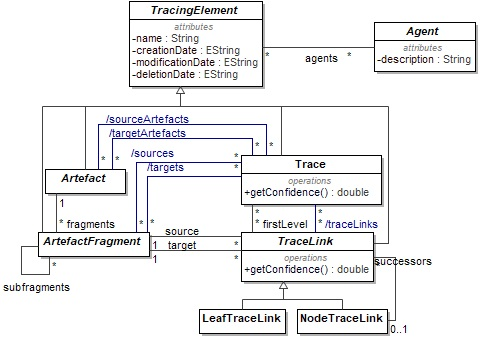
\includegraphics[width=.8\linewidth]{images/core.jpg}
	\caption{Core of Trace\textit{a}: Artefacts and (Trace)Links.}
	\label{fig:mm-core}
\end{figure}


\Fig{fig:mm-core} presents the core of the Trace\textit{a} language. At its center we find the notions of \textit{Trace}, \textit{link} (TraceLink), \textit{artefact} and \textit{fragment}. Links make up the traces and connect \textit{fragments} of the system to each other. We also notice the abstract nature of the Artefacts and Fragments. These are by definition volatile and must be redefined for each project or company to be best suited to concrete tracing needs.

\Fig{fig:mm-explainability} shows an extract from Trace\textit{a} specialized in the qualification of traces and links. The concepts of confidence (applied to Trace and TraceLink), as well as the creation, modification and deletion dates of the trace elements are present. These concepts make it possible to put in contact the evolution of the elements, their agent in charge (human or not) and the level of confidence linked to the traces and links. 

\begin{figure}[h]     
	\centering
	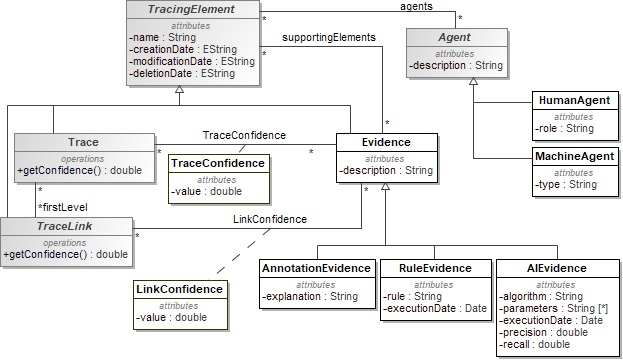
\includegraphics[width=.8\linewidth]{images/explainability.jpg}
	\caption{Excerpt of Trace\textit{a} dedicated to the quality of trace and link.}
	\label{fig:mm-explainability}
\end{figure}

Moreover, Trace\textit{a} allows the attribution to the traces of information (evidences) allowing their confidence values to be justified. Depending on the nature of the means of identification employed, these are an identification rule, a simple textual annotation, or the details of the training configuration and execution of a learning algorithm (classes at the bottom right corner). The execution parameters of the automated identification means (rules or learning algorithms) are thus available for consultation after their execution. The evidence may also point to supporting elements implicated in the calculation and justification of the level of confidence.


% \begin{figure}[h]     
% 	\centering
% 	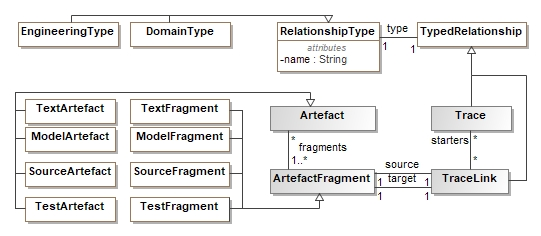
\includegraphics[width=.7\linewidth]{images/customization.jpg}
% 	\caption{Excerpt of Trace\textit{a} dedicated to the customization of traces and links.}
% 	\label{fig:mm-custom}
% \end{figure}




\subsubsection{The KerML/SysMLv2 ecosystem.}
\Fig{fig:kermlsysml} shows the architecture of the KerML / SysML ecosystem. The Kernel Modeling Language (KerML) formally defines a set of concepts allowing the development of languages specific to a given activity. 
% It is derived from three main classes: elements (Element), links (Relationship) and annotations (Annotation). These classes form the \textit{root} elements of the language (Root syntax) and are purely syntactic: they have no semantics related to modeling. These are linguistic elements allowing the construction of complex structures.
KerML has language elements defined at the syntax core level, themselves reusing the root language elements to allow the use of constructs specific to system modeling. These classes are redefined to establish the precise elements of modeling: relative to the construction of sequence diagrams, classes, activity, and the whole panoply of UML diagrams, among others. (For more details, see the KerML metamodel specification document ~\cite{kerML}).

\begin{figure}[ht]     
	\centering
	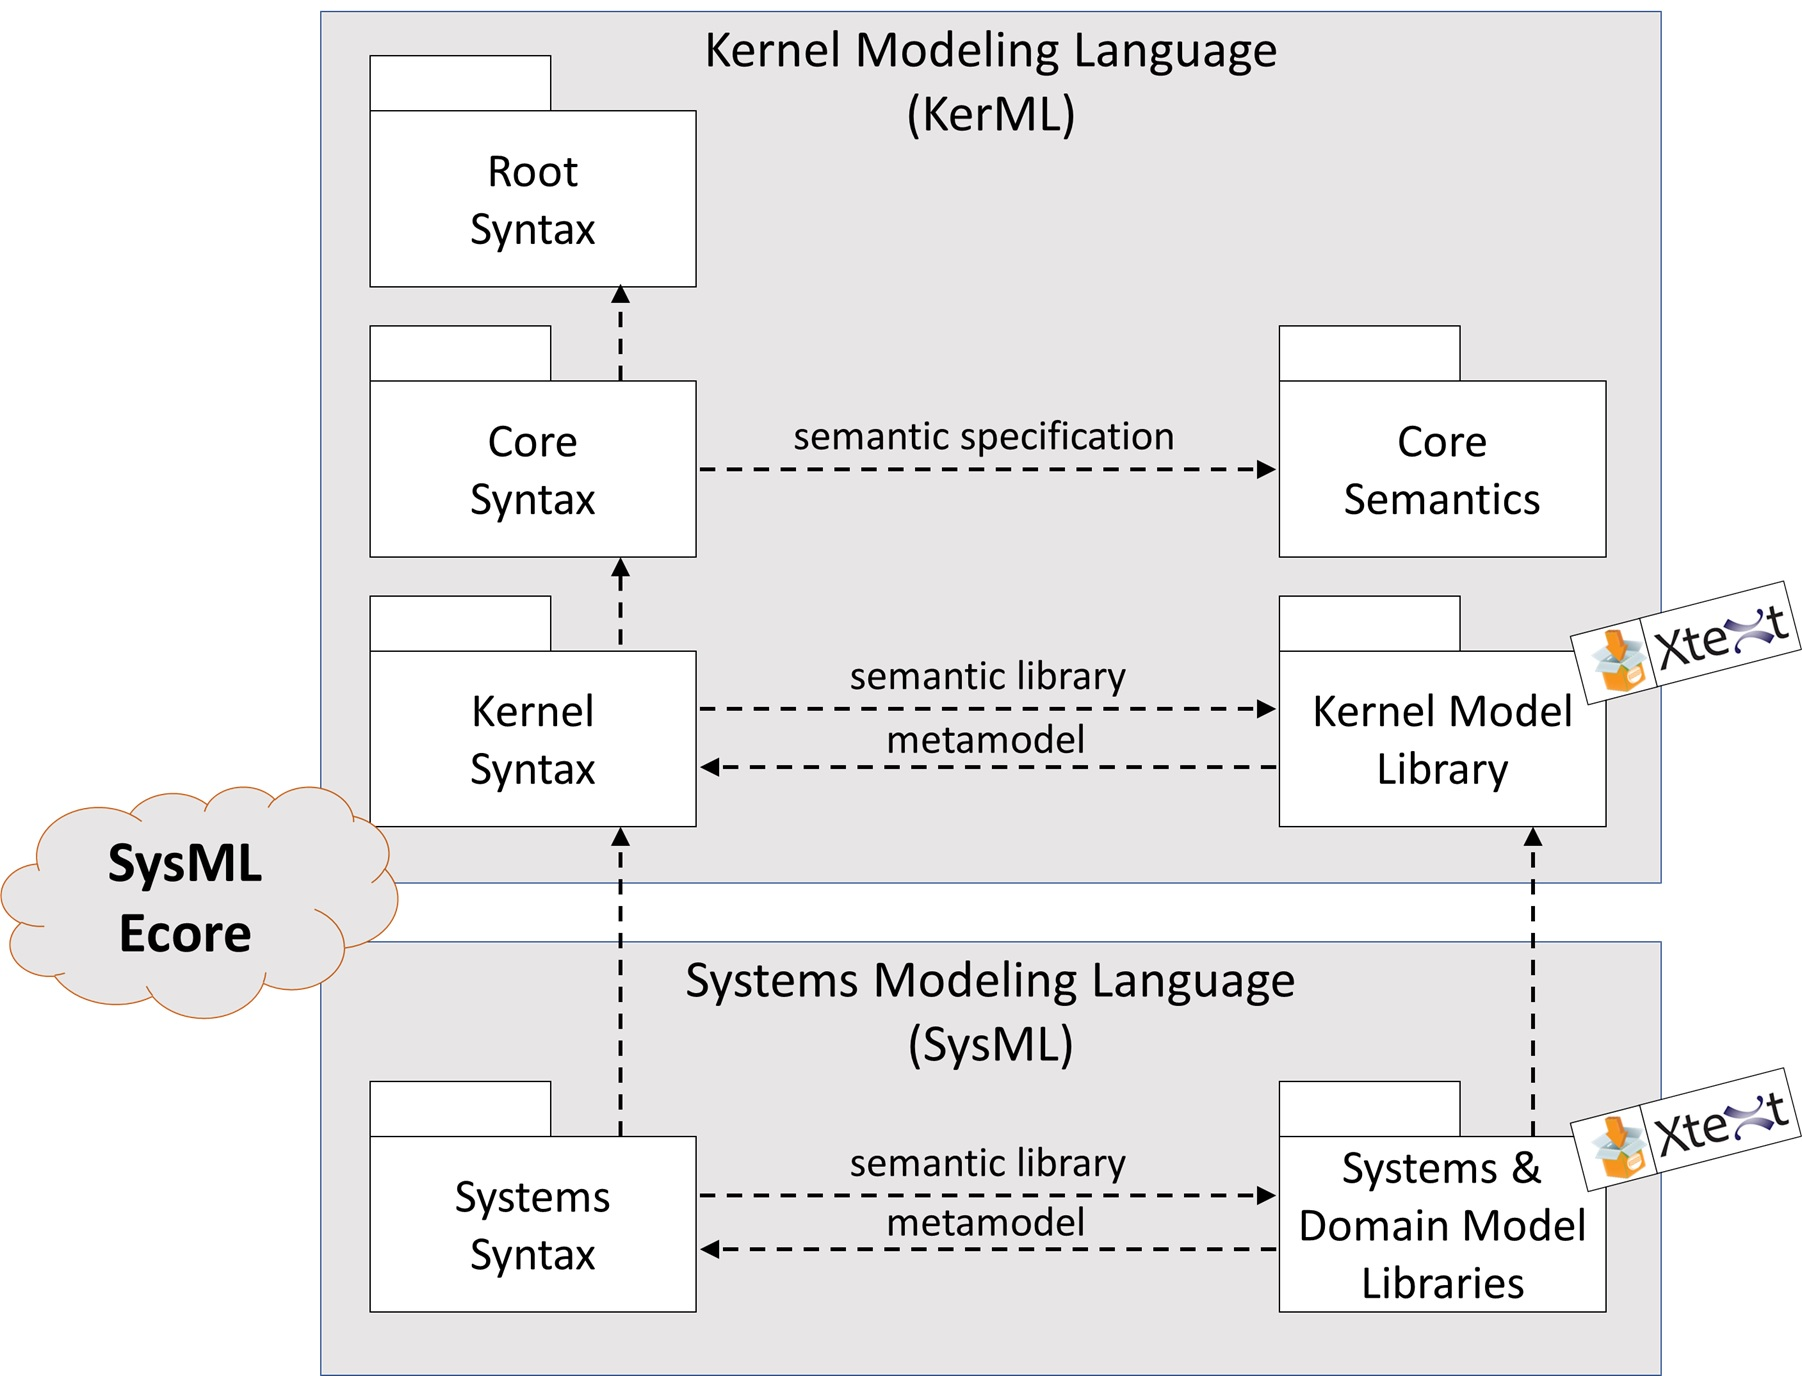
\includegraphics[width=.8\linewidth]{images/KerMLSysML.jpg}
	\caption{The KerML/SysMLv2 ecosystem.}
	\label{fig:kermlsysml}
\end{figure}



As shown in \Fig{fig:sysml}, the SysML language is constructed as an extension of the KerML Kernel metamodel ~\cite{kerML}. The SysML abstract syntax reuses the abstract kernel syntax, providing specialized constructs for modeling systems. Additionally, the SysML System Model Library extends the Kernel Model Library to provide the semantic specification for SysML. Finally, SysML provides an additional set of domain libraries to provide a rich set of reference models in various areas important for systems modeling (such as quantities and units, and basic geometry). (SysML p.69~\cite{sysml})

Finally, it is important to note that concrete elements of KerML cannot be instantiated from SysML.

\begin{figure}[ht]     
	\centering
	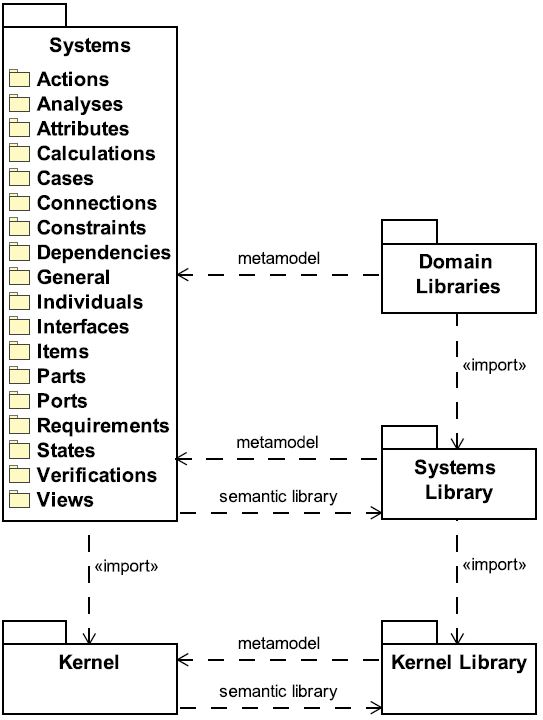
\includegraphics[width=.5\linewidth]{images/sysml.JPG}
	\caption{Architecture de SysML.}
	\label{fig:sysml}
\end{figure}

% \textit{\ugh{"}The Root layer is purely syntactic and has no modeling semantics. The Core is grounded in mathematical semantics (based on 7.3.1.2), supported by the Base package from the Kernel Model Library (see 8.2). The Kernel layer is given semantics fully through its relationship to the Model Library (see Clause 8). The semantic specification for each Kernel sub-package summarizes constraints on Kernel abstract syntax elements that specify how the model library is used when models are constructed following the abstract syntax.\ugh{"} (KerML p. 26)}

% \ughu{The [kerML] specification includes a metamodel that defines how models are structured (syntax) and model libraries that specify how real or virtual things are constructed or operated according to those models (semantics)~\cite{kerML}}.

% \begin{descriptioncompact}
%     \item[1 - KerML] Formal description of language elements
%     \item[2 - SysML] Adaptation to system development
% \end{descriptioncompact}

\subsubsection{Elements, Relationships, and Annotations}
KerML is organized around three fundamental concepts: Elements, Relationships and Annotations. The first two form the structure of the language and the third allows an orthogonal approach to it. Every element in SysML derives from these concepts.

\begin{figure}[ht]     
	\centering
	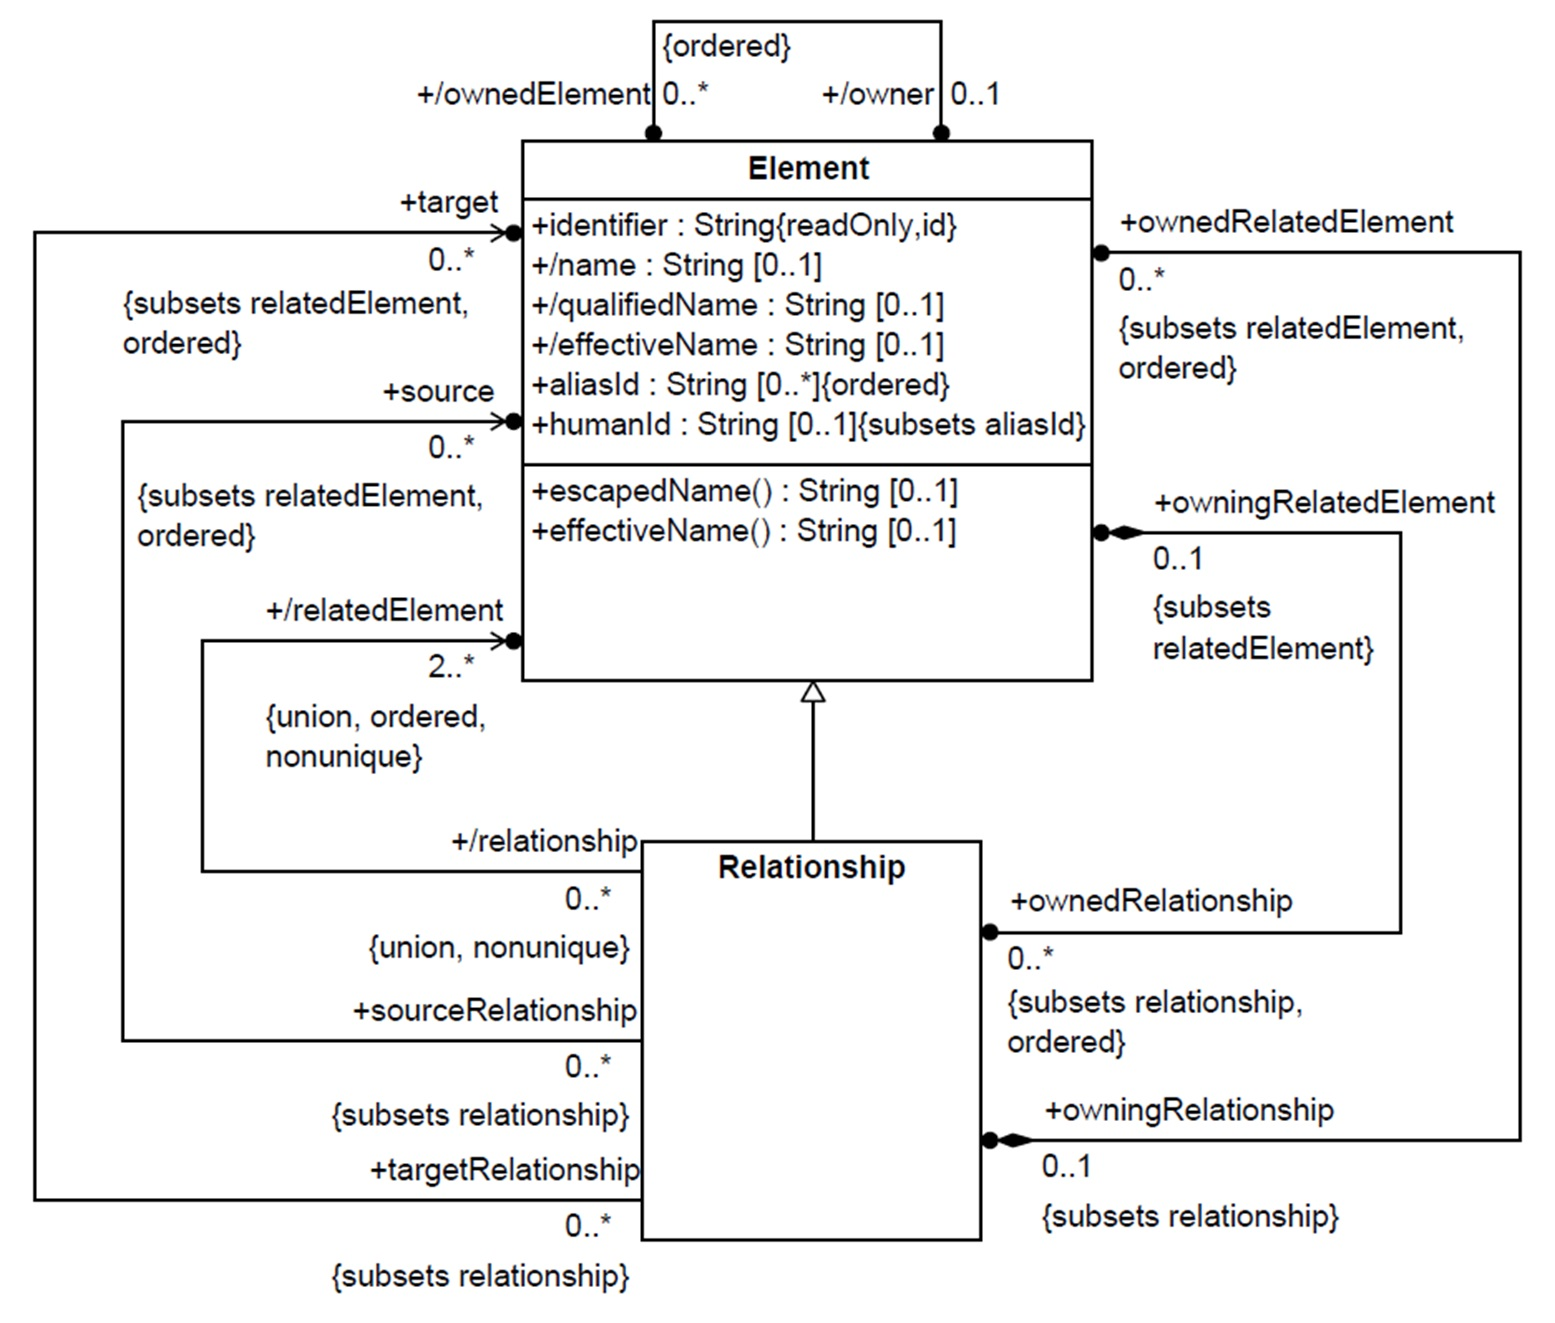
\includegraphics[width=.8\linewidth]{images/elementrelationship.jpg}
	\caption{Elements et Relationships dans KerML.}
	\label{fig:eltrel}
\end{figure}
More precisely, KerML makes it possible to represent complex structures in the form of graphs in which the nodes are Elements and the arcs are Relationships. Since a Relationship is itself an Element, relationship chains are also authorized and allow the nesting of features (\textit{nested features}). \Fig{fig:eltrel} specifies the links that exist between Element and Relationship. The \textit{ownership} is not detailed in this document but deserves to be mentioned here. Every Element is \textit{owned} by another. When one element is deleted, all the elements it \textit{owns} are also deleted.
For information purposes, Figures~\ref{fig:eltshierarchy} and~\ref{fig:relhierarchy} show the hierarchy derived from Elements and Relationships in KerML.

\begin{figure}[ht]     
	\centering
	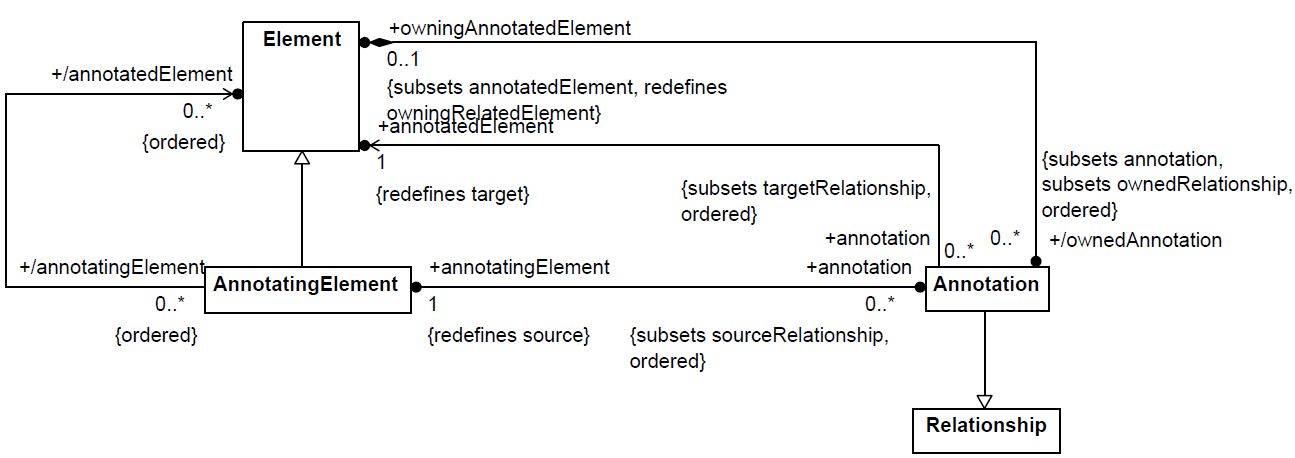
\includegraphics[width=.99\linewidth]{images/annotations.JPG}
	\caption{Annotations in KerML.}
	\label{fig:annot}
\end{figure}

On the other hand, "an Annotation is a relationship between an element and an AnnotatingElement that provides additional information about the annotated element. Each annotation falls between a single AnnotatingElement and a single element being annotated, but an AnnotatingElement can have multiple annotation relationships with different annotatedElements, and any element can have multiple annotations." (KerML Specification, p. 37~\cite{kerML}).

In the case of traceability, annotations can be used to identify types of links and tag \textit{relevant} links (\textit{i.e.,} according to the specific use we want to make of them). We will speak of an \textit{orthogonal} approach by annotations. 
\vspace{5em}
\begin{figure}[ht]     
	\centering
	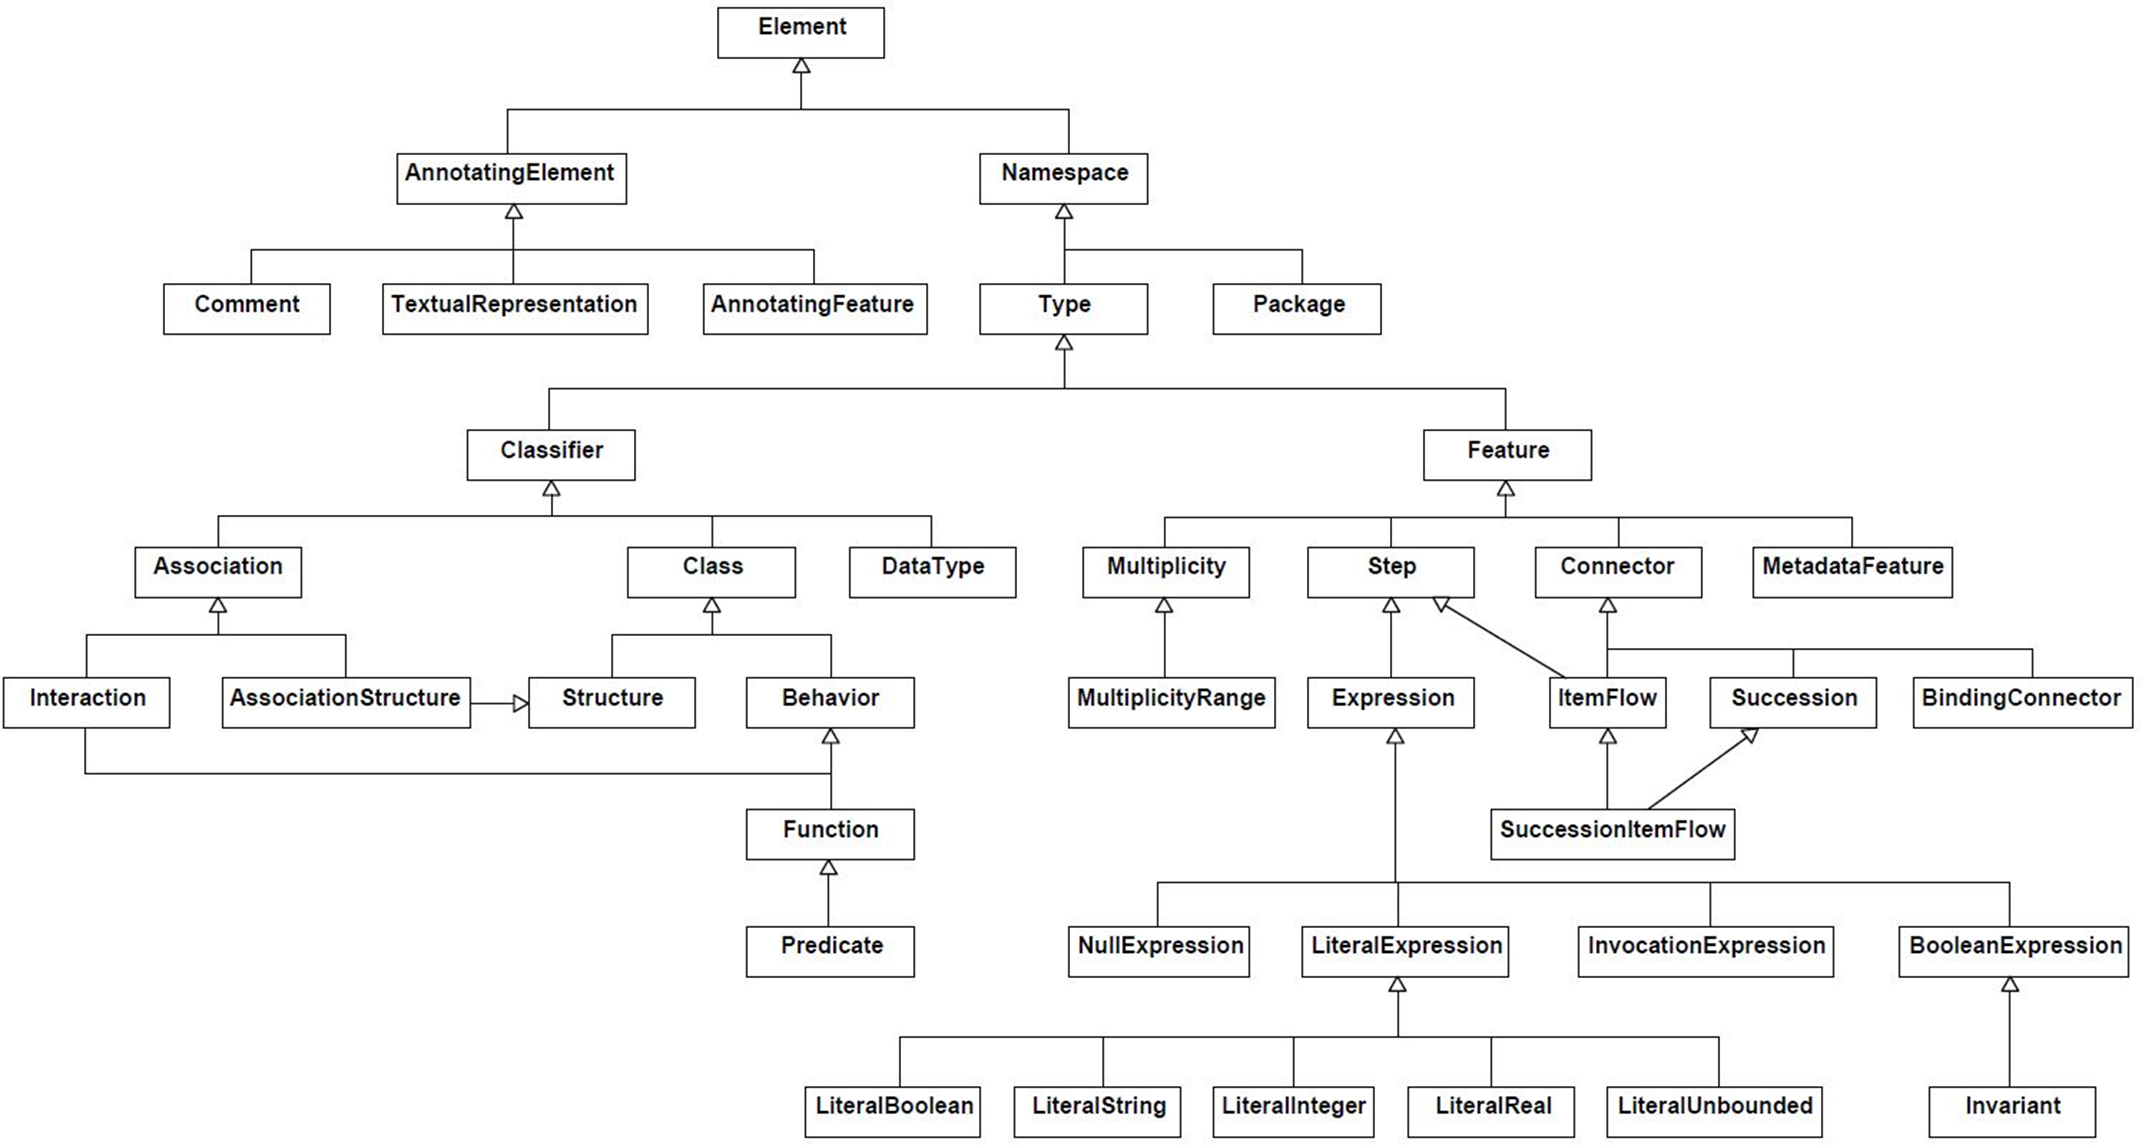
\includegraphics[width=.99\linewidth]{images/kerml-element.png}
	\caption{Hierarchy of KerML Elements.}
	\label{fig:eltshierarchy}
\end{figure}

\begin{figure}[ht]     
	\centering
	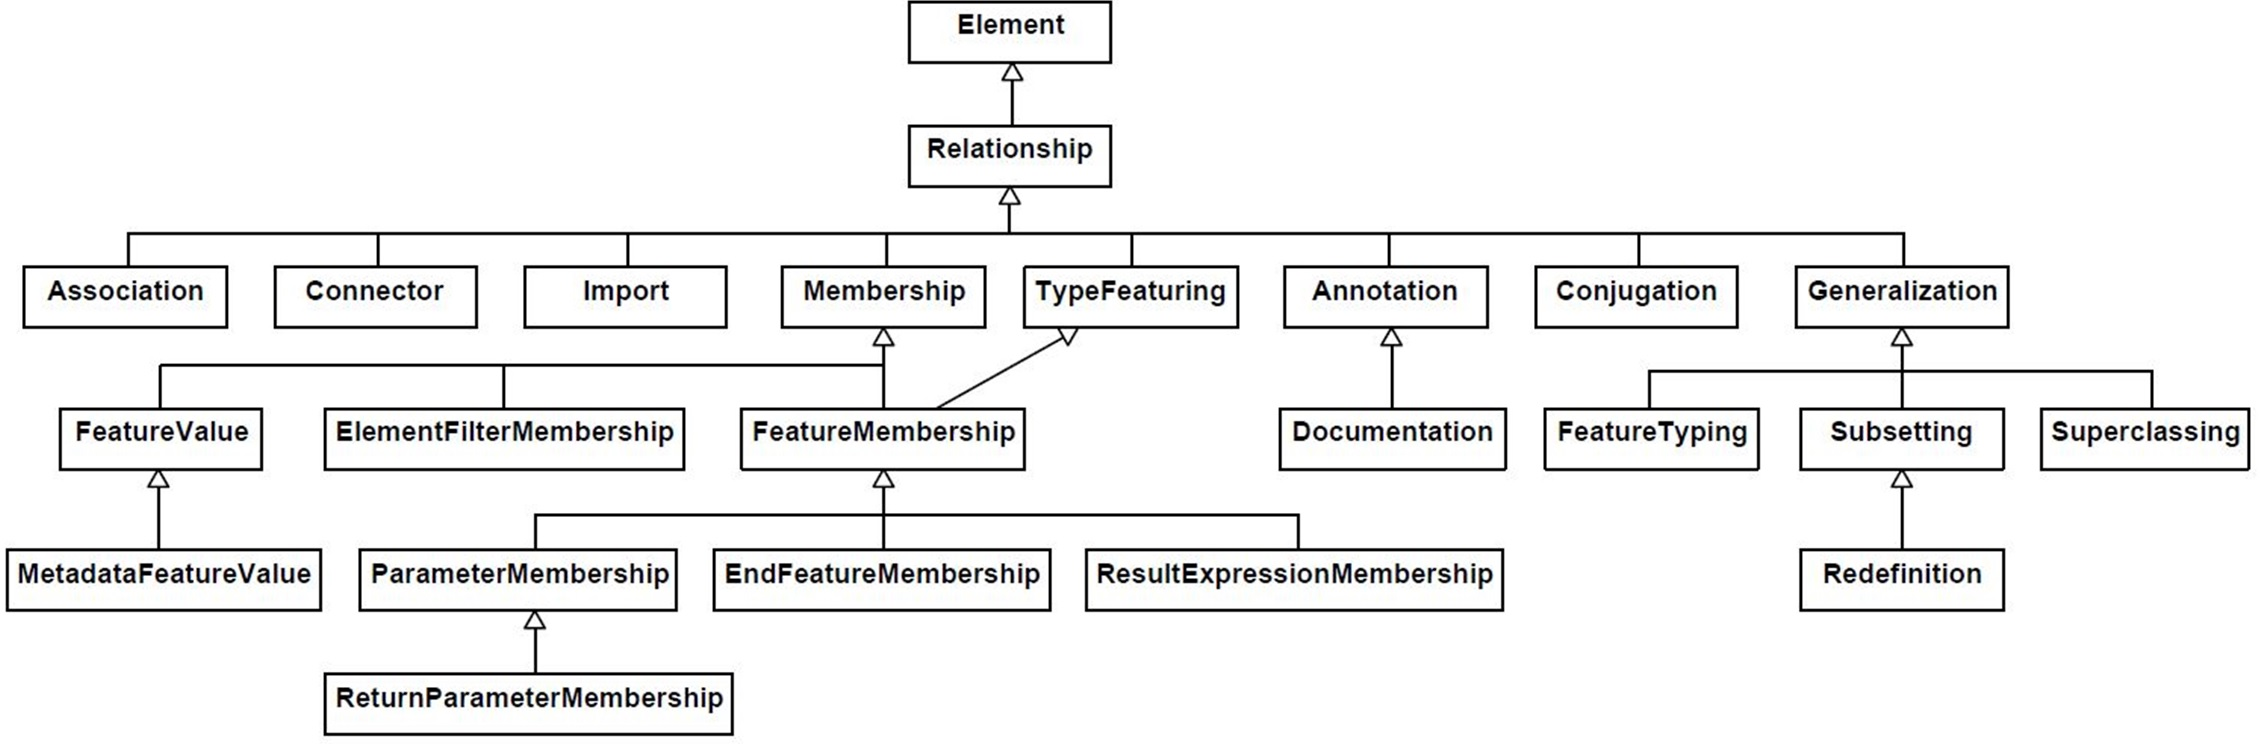
\includegraphics[width=.99\linewidth]{images/kerml-relationship.jpg}
	\caption{Hierarchy of KerML Relationships.}
	\label{fig:relhierarchy}
\end{figure}


% \begin{descriptioncompact}
%     \item[Elements] Top level (root) element of the KerML language.
%     \item[Relationships] Links between elements.
%     \item[Annotations] Open window to orthogonal considerations.
% \end{descriptioncompact}


\subsection{Goals}
The needs in terms of traceability have been established in Deliverable 1 ~ \ cite {deliverable1}. We summarize here the high level needs to satisfy a quality traceability, \textit{i.e.,} allowing to qualify quantitatively and qualitatively the identified links useful for the tracing.
    
\subsubsection{Mastering complexity}
The tracing must allow to measure or approximate the complexity of the system. Since the concept of "Complexity" suffers from a high degree of volatility, its measurement (or its \textit{proxy}) requires a consequent adaptability.
    
\subsubsection{Increase the ability to scale the system}
To facilitate the monitoring of the evolution of the system over time, tracing makes it possible to concentrate the measurement of the impact (\textit{eg,} of a change) on (types of) specifically chosen links.
    % \ item [Independence from target system]
    
\subsubsection{Maintain a degree of independence from the target system}
Tracing must not influence the system. It must remain independent, or \textit{orthogonal}, so that \textit{i)} it does not alter the evolution of the system, \textit{ii)} it does not depend on decisions relating to the development of the system, and \textit{iii)} it remains possible to plot systems of systems (\textit{ie,} written in different languages, on different platforms).% \end{descriptioncompact}


\section{Strategies for traceability of SysML elements}\label{sec:strategies}
\sideboxbegin{o}
This section presents the 4 strategies considered to integrate the functionalities of Trace\textit{a} into SysMLv2.
\sideboxend

During this fourth deliverable we explored  different strategies offered by SysML to allow trustable traceability.

In this section, we present the four strategies considered, their strengths and weaknesses, as well as the one promoted by those in charge of the SST.
This section details the integration of the concepts of trace and trace link within KerML to be able to harness the notions of confidence and justifications (Evidence) of these latter. 
 
\subsection{Root-level adaptations}
\begin{figure}[h]     
	\centering
	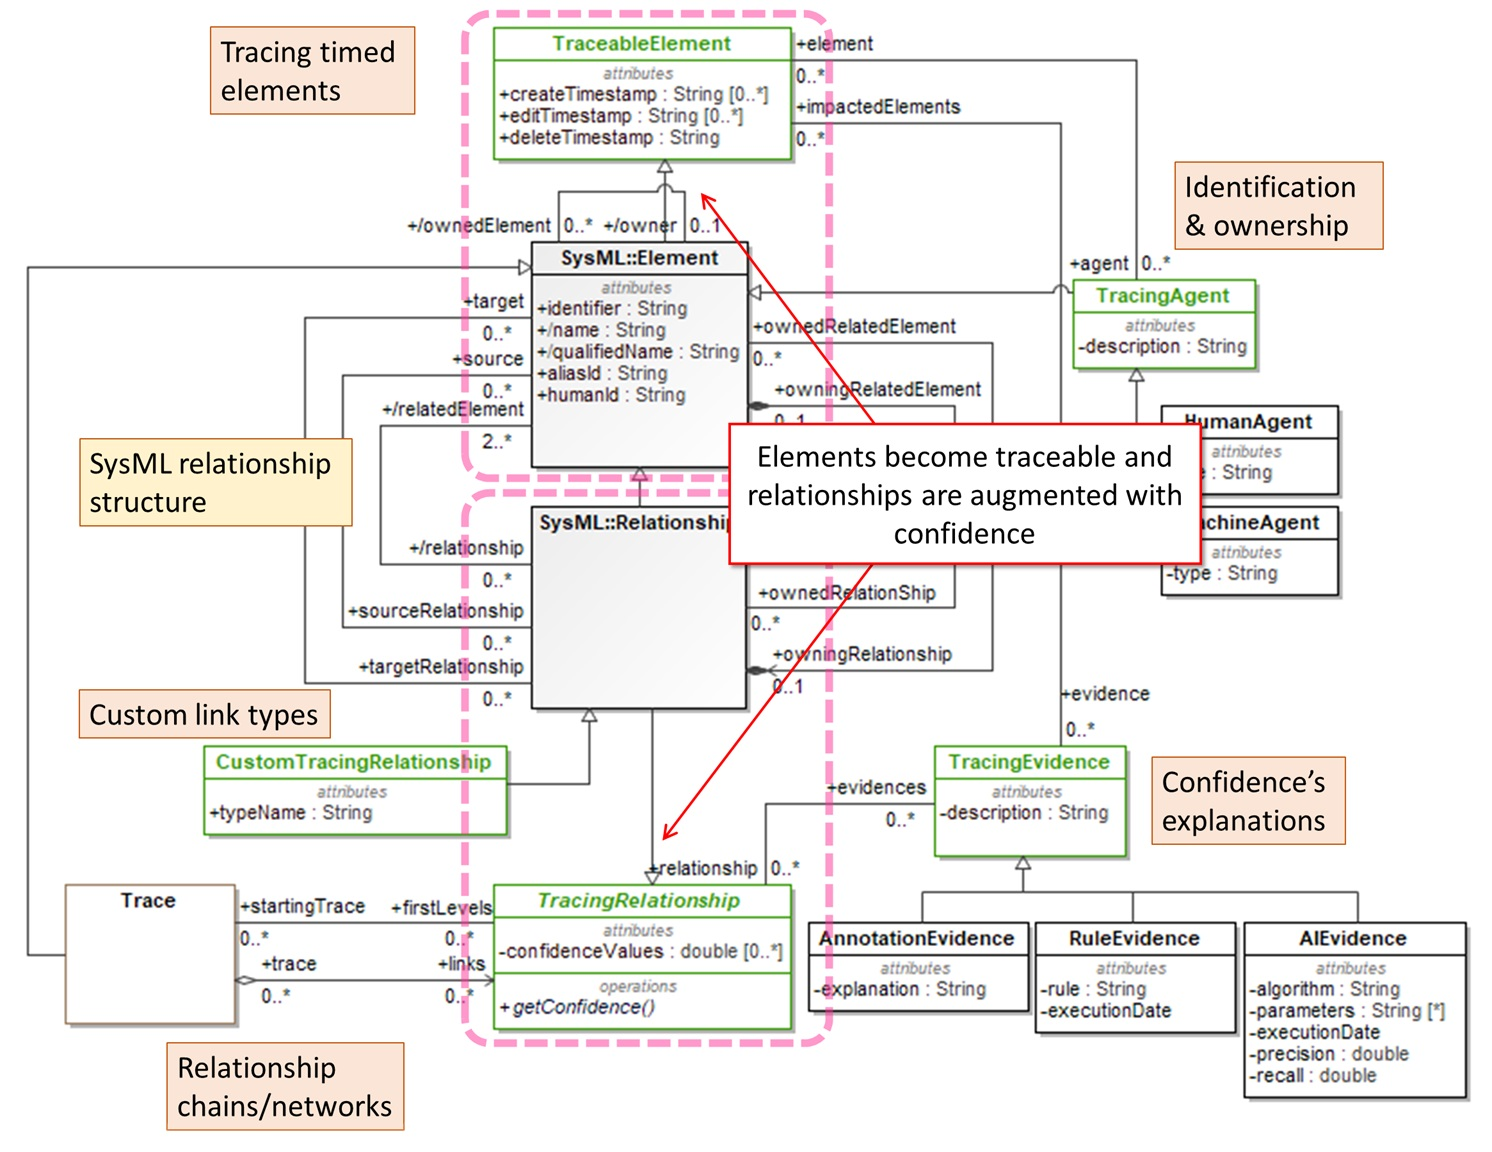
\includegraphics[width=.95\linewidth]{images/strategy1-root.jpg}
	\caption{Adaptation of root-level elements. }
	\label{fig:strategy1}
\end{figure}
The first strategy consists in augmenting the root elements with the attributes necessary for traceability. \Fig{fig:strategy1} shows the modifications required. In gray are the SysML classes, in green the hinge/border classes. The purple dotted lines underline the areas of interest. A TraceableElement class increases the {KerML} Elements by aggregating evolution markers (timestamps) and references to the agents responsible for their identification. The latter are particularly interesting when using non-deterministic algorithms for identifying the tracing links (see the detail of the metamodel of Trace\textit{a} for more details~\cite{batot2021-not-another-metamodel}).
Another class comes to increase the Relationships by attributing to it a value of confidence.

This strategy must have been left because it turns out to be too intrusive in the language. Changing the root elements potentially impacts the entire language structure and therefore could not be incorporated into the KerML/SysMLv2 specification process. Moreover, this strategy implies the definition of a concrete syntax which fits into the {KerML} language schema -- which can be very expensive in terms of consistency evaluation and verification.

\subsection{Annotation type dedicated to tracing}
\begin{figure}[ht]     
	\centering
	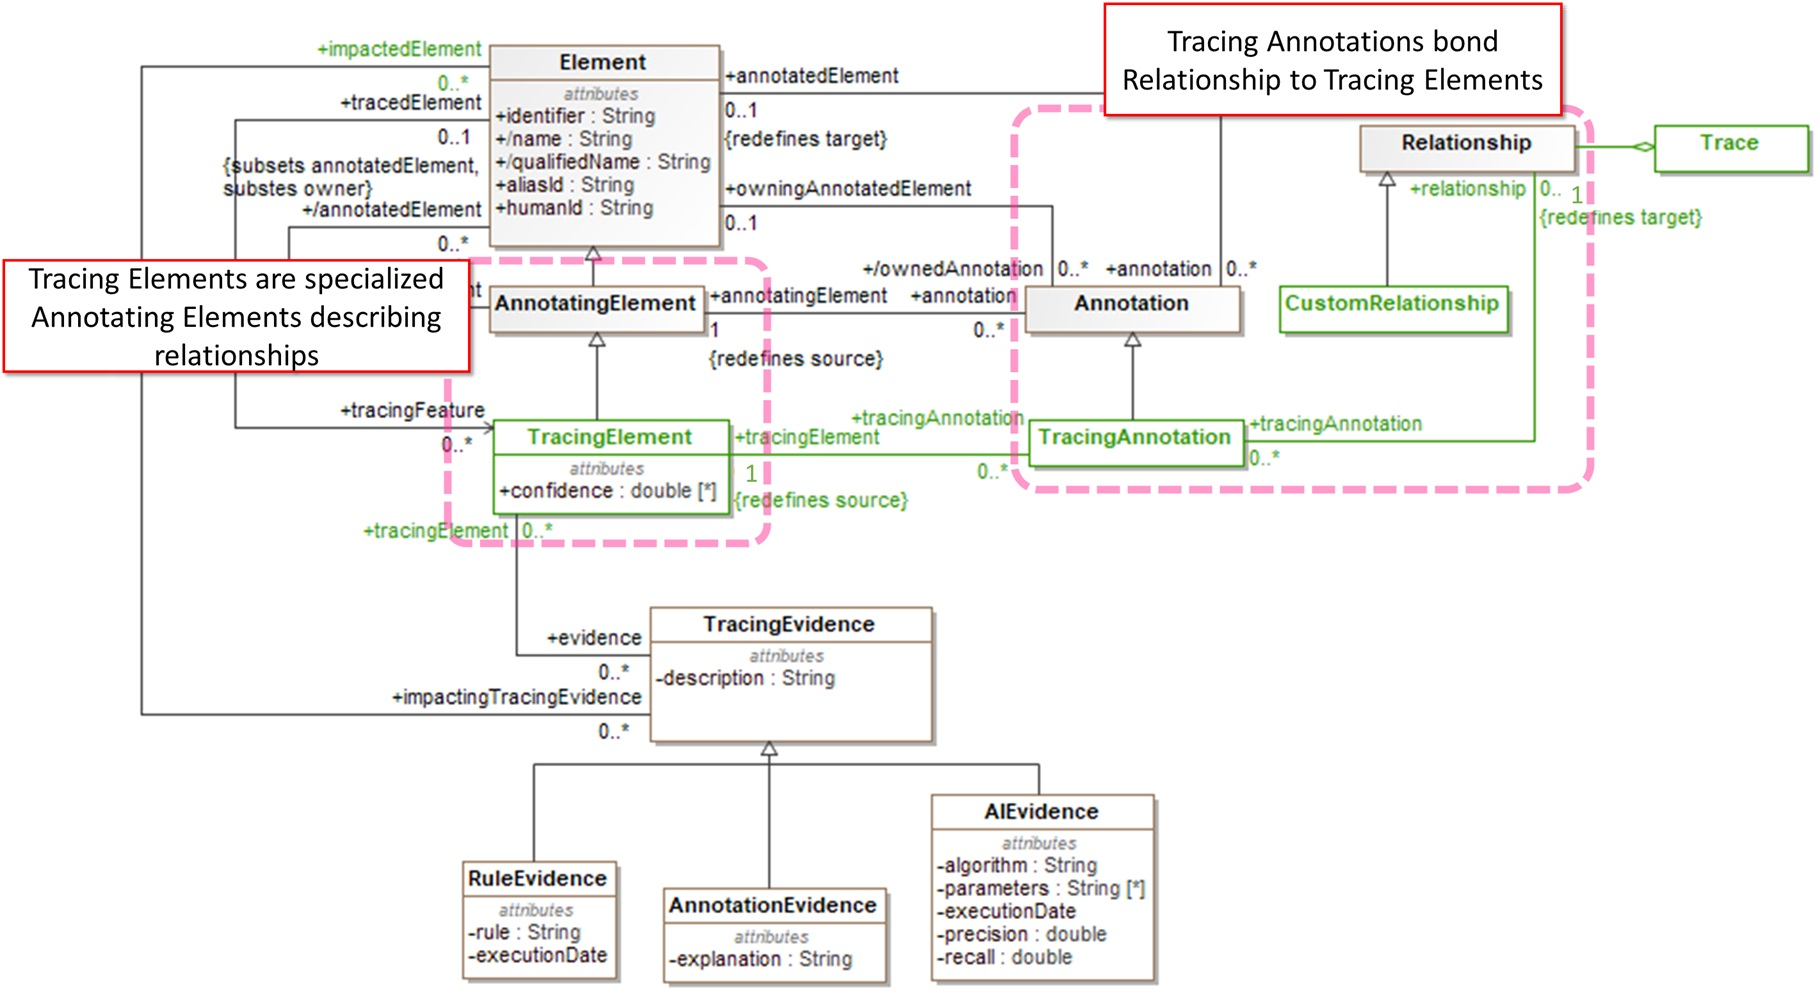
\includegraphics[width=.99\linewidth]{images/strategy2-annotation.jpg}
	\caption{A new type of annotation for {KerML}.}
	\label{fig:strategy2}
\end{figure}
To avoid modifying the fundamental elements of {KerML}, our second idea was to redefine an annotation type dedicated to tracing. To do this, a TracingAnnotation links a Relationship to a TracingElement just as an annotation links an Element to an AnnotatingElement. The idea is to allow the relevant relationships to be annotated with confidence values (and associated with a set of information justifying the calculation of these values). \Fig{fig:strategy2} illustrates the modifications necessary to apply this extension to {KerML}.

This strategy reuses the existing concrete syntax (and to add the keywords necessary to enter the confidence value and the justifications). An illustrative example is provided in Listing~\ref{lst:strategy1}.
However, this strategy poses a problem {in terms of tooling}. Indeed, by modifying the abstract syntax (the metamodel) to add a new type of annotation, all the tools allowing the manipulation of this syntax must be updated.
{This is an intrusive solution again. In a language still in the process of stabilization, the chances of making these changes happen are slim.}
% \vspace{4cm}

\begin{center}
\begin{lstlisting}[caption={Sample of a concrete syntax for tracing annotations},
label=lst:strategy1,
style=mystylesysml,
linewidth=12.5cm,
xleftmargin=4.2cm,
morekeywords={type,confidence,description}]
  trace Req2Source {
     from elt1 to elt2 /** Elements */ 
     type CustomLinkForClasses
     confidence 0.83
     impacts D, E, F
     description "Something"
  }
\end{lstlisting}
\end{center}  


% \vspace{6cm}
Nonetheless, the concept of annotation is to be retained here -- it suits perfectly the idea of traceability \textit{orthogonal} to the software. With tracing annotation, a change in the traced elements does not necessarily impact the tracing elements, and vice versa.



\subsection{A new type of (\textit{annotating feature)}}
\begin{figure}[h]     
	\centering
	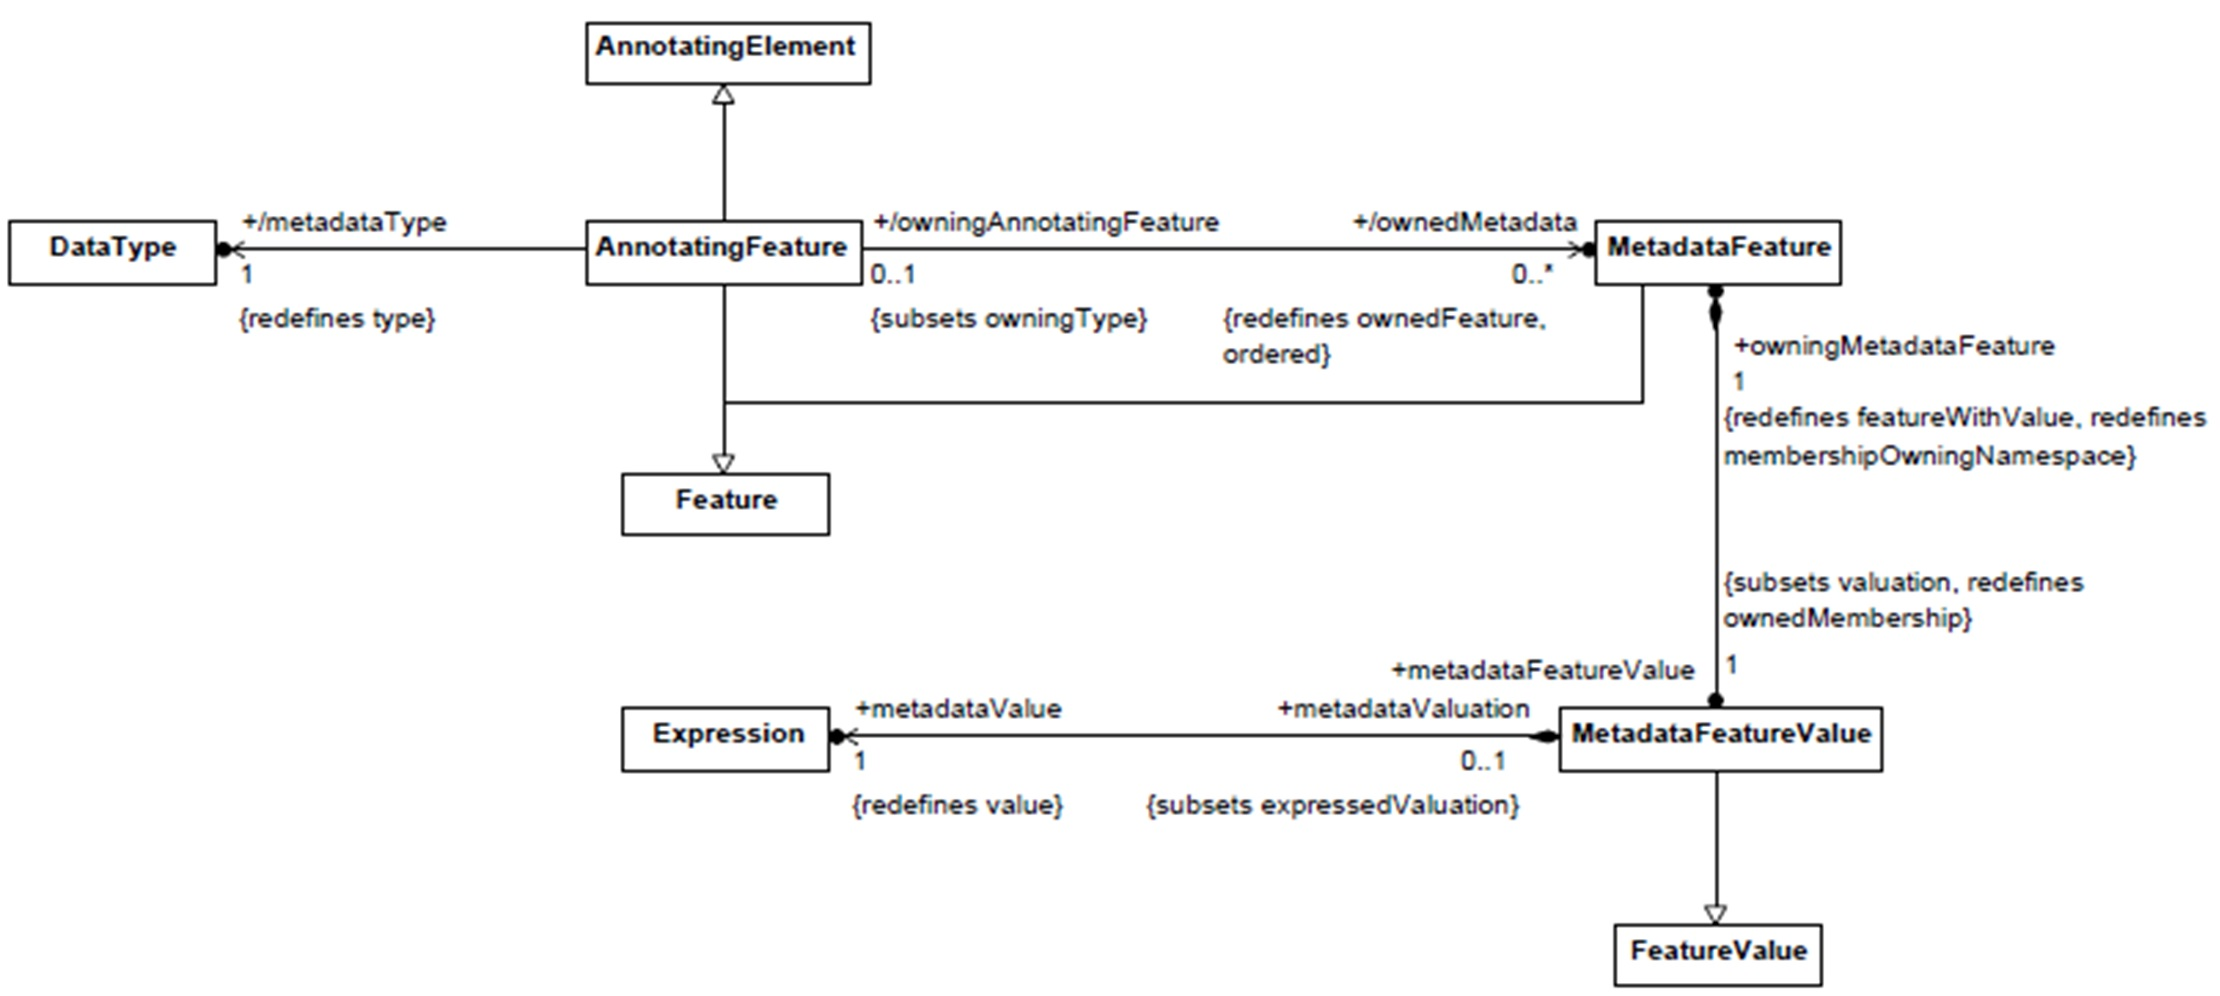
\includegraphics[width=.99\linewidth]{images/kerml-annotatingfeature.jpg}
	\caption{Snippet of the KerML metamodel: AnnotatingFeature and valued Expressions for adaptable metadatatypes.}
	\label{fig:kermlannot}
\end{figure}

\begin{figure}[h]     
	\centering
	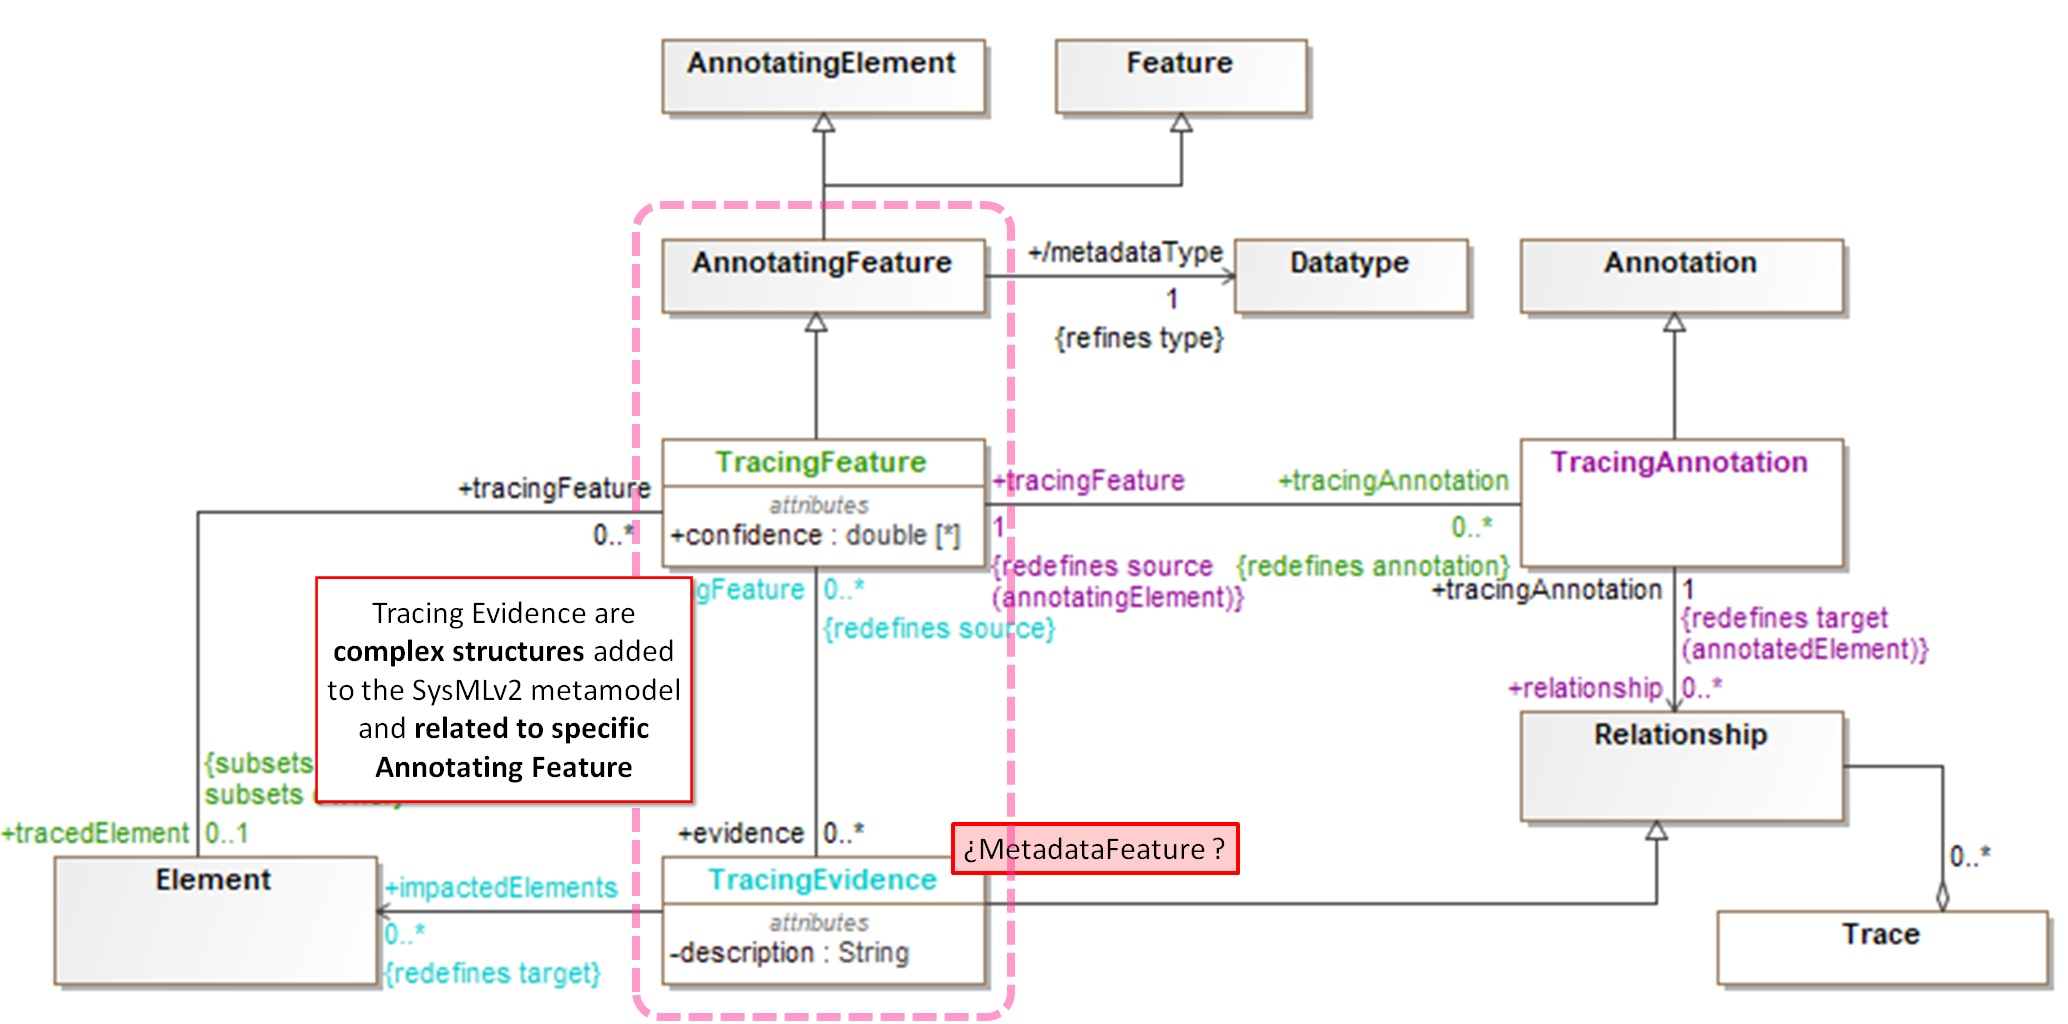
\includegraphics[width=.99\linewidth]{images/strategy3-annotatingfeature.jpg}
	\caption{A new type of annotating feature dedicated to traceability .}
	\label{fig:strategy3}
\end{figure}

The KerML specification states that "\textit{an AnnotatingFeature is a kind of AnnotatingElement that allows the definition of structured metadata with attributes specified by the modeler.}" (KerML specification, p. 178~\cite{kerML}). \Fig{fig:kermlannot} presents a snippet of the KerML metamodel where the AnnotatingFeature class is defined. AnnotatingFeatures use MetadataFeatures which redefine new features for associated elements (respecting the typing defined in DataTypes). These features will be evaluated at the \textit{execution of expression at model level} and a value will be associated with each feature.

\Fig{fig:strategy3} shows the modifications to be made to {KerML} to allow the redefinition of a new type of AnnotatingFeature dedicated to traceability.
A TracingAnnotation associates a TracingFeature with a Relationship. This Feature includes a level of confidence and possibly evidence (references to other elements).



This approach is the most interesting. KerML / SysMLv2 maintainers informed us that this "AnnotatingFeature / Datatype" structure is in their sights because it allows the addition of functionality in the form of metadata libraries without directly modifying the language elements (what we call "orthogonality" ). More precisely, they plan to use only this type of annotation and to ban its refinement in favor of this structure to allow the simplified writing of specialized function libraries (\textit{feature libraries}).
From September 2021, the different types of AnnotatingElement (Comment, TextualRepresentation and AnnotatingFeature) will converge to a representation based on AnnotatingFeature. This migration will simplify, first of all, the elaboration of comments specific to a project / domain thanks to the use of dedicated Datatypes.

% \pagebreak
\subsection{A feature library for traceability }
The last strategy considered will be the one implemented. Instead of modifying the abstract syntax structure of {KerML} (\textit{i.e.,} metamodel level), the idea is to create a library of features dedicated to traceability (model level).
It is about redefining datatypes specific to the tracing features in order to join them to the structures concerned at the model level. It is an orthogonal method comparable to the use of \textit{stereotypes} in UML. The comparison is based on the ability offered by the AnnotatingFeature to define new (libraries of) features without altering the base of the language itself. The process is particularly suited to building a tracing strategy, often implemented \textit{after} the software has been put into production.

\vspace{3em}
The Listings \ref{lst:featurelibrary1} and \ref{lst:featurelibrary2} present our feature library {in SysML}. Listing~\ref{lst:featurelibrary1} contains the library declaration; Listing~\ref{lst:featurelibrary2} contains an example of application of such datatype  defined on a concrete example. It illustrates the allocation of a confidence value of 0.7 to a connection between a requirement (req) and a package. The second case (line 16 to 20) attributes a description and points to an element impacted (by the evaluation of the confidence),
% \vspace{10cm}

\begin{center}
\begin{lstlisting}[caption={Definition of a datatype dedicated to traceability (partial listing).},
label=lst:featurelibrary1,
style=mystylesysml,
linewidth=15cm,
xleftmargin=2.2cm,
morekeywords={part,filter}]
 package TracingAnnotations {
	attribute def ConfidenceTracing {
		attribute confidence : Real;
		attribute impact : Anything[*]
		assert constraint 
		  { confidence >= 0.0 && confidence <= 1.0 } 
	}
	 
	attribute def ExplainableTracing {
		attribute description : String;
		attribute evidence : Evidence;
		attribute agent : Agent;
	}  
 }
\end{lstlisting}
\end{center}  

\begin{center}
\begin{lstlisting}[caption={Use of metadata features for traceability},
label=lst:featurelibrary2,
style=mystylesysml,
frame=shadowbox,
rulesepcolor=\color{blue},
linewidth=15cm,
xleftmargin=2.2cm,
morekeywords={confidence,description,evidence,impact, part, req,package}]
 import package TracingAnnotations::*;

 /*Definition of the target system. */
 part vehiculetest {}
 req RE01_MLV {}
 package UMLCD_CORE {}

 /*Assignment of a confidence of 0.7 to the Req2Design link.*/
 connection Req2Design connect RE01_MLV to UMLCD_CORE {
   @ConfidenceTracing {
     confidence = 0.7;
   }
 }
 
 /*Assigning a description and an impact to the Req2Design link.*/
 connection Req2Design connect RE01_MLV to UMLCD_CORE {
   @ExplainableTracing {
     description = "Something";
     impact = (vehiculetest);
   }
 }
 
\end{lstlisting}
\end{center}


% 
\begin{center}
\begin{lstlisting}[caption={Confidence and evidences for trustable traceability},label=lst:relationship,style=mystylextext,frame=shadowbox, rulesepcolor=\color{blue}]
Relationship  returns SysML::Relationship :
    'relationship' Identification?
    RelationshipRelatedElements
    RelationshipBody;

OwnedRelationship returns SysML::Relationship :
    'relationship' Identification?
    'to' RelationshipTargetList
    RelationshipBody;

fragment RelationshipRelatedElements 
            returns SysML::Relationship :
    'from' RelationshipSourceList ( 'to' RelationshipTargetList )?
  | 'to' RelationshipTargetList;

fragment RelationshipSourceList returns SysML::Relationship :
    RelationshipSource ( ',' RelationshipSource )*;

fragment RelationshipSource returns SysML::Relationship :
    source += [SysML::Element | QualifiedName];

fragment RelationshipTargetList returns SysML::Relationship :
    RelationshipTarget ( ',' RelationshipTarget )*
;

fragment RelationshipTarget returns SysML::Relationship :
    target += [SysML::Element | QualifiedName];

fragment RelationshipBody returns SysML::Relationship :
    ';' | '{' RelationshipOwnedElement* '}';

fragment RelationshipOwnedElement returns SysML::Relationship:
      ownedRelatedElement += OwnedRelatedElement
    | ownedRelationship += OwnedDocumentation
    | ownedRelationship += OwnedTextualRepresentationAnnotation;

OwnedRelatedElement returns SysML::Element :
      'element' ( humanId = Name )? ElementBody
    | OwnedRelatedRelationship;

OwnedRelatedRelationship returns SysML::Relationship :
    'relationship' ( humanId = Name )? RelationshipBody;
\end{lstlisting}
\end{center}


\section{Metadata feature library for quality traceability}\label{sec:extension}

\sideboxbegin{o}
This section presents the limitations imposed by the state of the art of KerML / SysMLv2 in terms of meta-annotation. It then presents the design that we have implemented to overcome it.
\sideboxend
We have previously mentioned the advantages that the use of feature libraries  (orthogonal) offers compared to more intrusive strategies (modifying the structure of the language).

However, the development of datatypes dedicated to traceability encounters a certain number of limitations due to the state of progress of the implementation of KerML / SysMLv2. In this section, we present the limitations encountered and then our design for quality traceability for KerML \textit{and} SysMLv2.

\subsection{Orthogonality - priority and limitations}\label{sec:orthogonalite}
 
\begin{figure}[ht]     
	\centering
	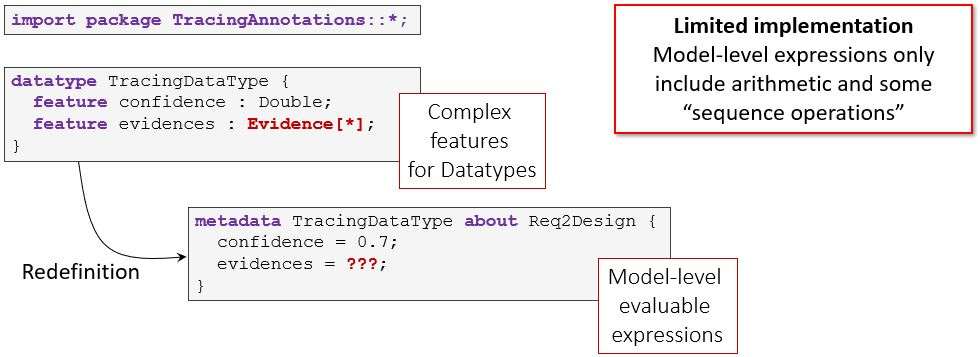
\includegraphics[width=.99\linewidth]{images/strategy4-metadatatype.jpg}
	\caption{Defining complex Metadata structures and evaluating expressions at model level: implementation limits. }
	\label{fig:strategy4}
\end{figure}


To use the words of Ed Seidewitz, one of the main promoters of the new version of SysML and one of the main people responsible for its delivery, the idea of using the AnnotatingFeatures to define \textit{a priori} external needs to the language specifications is "extremely relevant". However, the next revision will not contain any specific article on the matter. A number of decisions remain to be clarified on the subject.
In particular, the ability to define and reuse complex structures within feature datatypes is under consideration. For now, the definition of complex datatype is not guaranteed to work, as illustrated in \Fig{fig:strategy4}.

\begin{figure}[ht]     
	\centering
	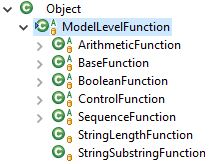
\includegraphics[width=.35\linewidth]{images/modellevelfunction-type-hierarchy.JPG}
	\caption{Types of functions available for evaluating expressions at the model level.}
	\label{fig:modellevelfunc}
\end{figure}

Until the delivery of the second revision (RFP2) scheduled for late August 2021, the SST remains busy with other priorities. Ed Seidewitz foresees the deployment of the features related to modelv level expression in October or November 2021. At the time of writing, annotating features are "only" templates in which some points of variability are allowed (the authorized functions are derived from ModelLevelFunction, see \Fig{fig:modellevelfunc}).

Consequently, the definition of complex structures within datatypes is limited as stated above. Only Ed Seidewitz is aware of the code related to the question and he himself struggles to remember the state of the module dedicated to the assignment of values to complex datatypes. As an example, the use of enumeration (\textit{enum}) in annotations does not allow their use for evaluation (see \Sect{sec:filter}). 
Finalizing this implementation will only be possible when a subset of the modeling language SysML will be defined. In view of the SST's plans to converge the different types of annotations towards AnnotatingFeatures using metadatatypes, these points will be addressed with high priority -- but only after the submission of the new revision.

\subsection{Iterative design: confidence and explainability of trace links}\label{sec:design}
\begin{figure}[ht]      
	\centering
	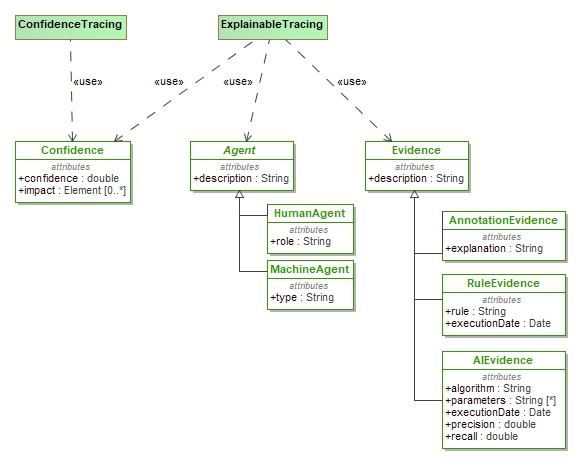
\includegraphics[width=.9\linewidth]{images/explainability-datatype.jpg}
	\caption{Metadatatypes for quality traceability including an assessment of confidence and monitoring of the identification processes used.}
	\label{fig:datatypes}
\end{figure}

To favor the use of specialized libraries (such as the SST encourages), we have designed SysML and KerML datatypes dedicated to tracing. 
\Fig{fig:datatypes} shows the design of these structures. At the top, we distinguish between a design allowing the assessment of confidence and a design allowing to go further by entering the supporting information for this assessment.
We distinguish between the two for the sake of iterativity of the development and implementation processes (as we have just seen, the mechanisms allowing the manipulation and evaluation of datatypes are not fully completed in KerML / SysMLv2).

The \texttt{ConfidenceTracing} datatype has been implemented to overcome this disappointment and initially allows the attribution of a real value of confidence to the annotated links. We add a description field (free String) and a field to reference to potentially impacted elements -- \textit{e.g.,} used in the calculation of the confidence value.
The \texttt{ExplainableTracing} datatype has the same attributes as ConfidenceTracing (description, confidence and impact) with in addition \textit{i)} the notion of Evidence to store information about the identification process used for tracing, and \textit{ii)} the possibility to inform which (type of) agent is responsible for identification.

\subsection{Consequence of the separation of KerML and SysML languages}\label{sec:lggsep}
SysML is based on KerML. However, if the language dedicated to systems reuses the concepts of the kernel language, these are not accessible from the former. Thus, the definition of a Datatype (and its associated Features) does not work in SysML but only in KerML. To allow the use of Trace\textit{a} in both languages, we have transformed the Datatypes and their features into \textit{attribute definitions and uses} (resp. "Attribute def" and "Attribute"). Indeed, an attribute definition is a particular type of structure dedicated to the construction of Datatypes for the design of systems (see \Fig{fig:dtnattributes}).


\begin{figure}[h]     
	\centering
	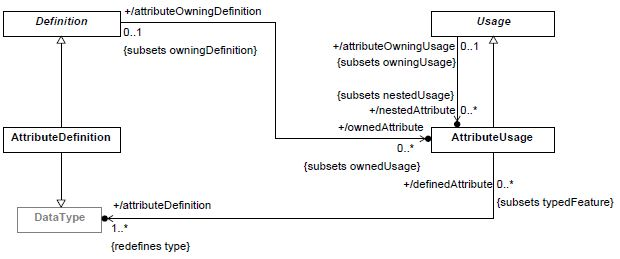
\includegraphics[width=.9\linewidth]{images/dtnattributes.JPG}
	\caption{The definition and use of attributes in SysML is a specialization of datatypes and their features in KerML.}
	\label{fig:dtnattributes}
\end{figure} 

\subsection{Usage example: filtering}\label{sec:filter}
This section presents an example: the filtering of links satisfying a confidence greater than a given threshold.
The first 30 lines of listing~\ref{lst:filter} (with graphical representation in \Fig{fig:vizfilter}), show the structure of the system and links being traced. Lines 33 to 39 show the code needed for filtering. This is a reuse of the existing machinery to support SysMLv2 metadata annotations. \Fig{fig:vizfilterres} shows the result of the query: the five links with a confidence greater than 0.5 are filtered.

% \pagebreak
\begin{lstlisting}[caption={Definition and filtering of tracing annotations to collect links satisfying a certain level of confidence.},
label=lst:filter,
style=mystylesysml,
linewidth=16cm,
xleftmargin=1.7cm,
morekeywords={part,filter}]
package Tracing_FilterExample {
	import TracingAnnotations::*;
	
	/* System under tracing. */
	part end1 {}
	part end2 {}
	part end3 {}
	part end4 {}
	part end5 {}
	part end6 {}
	part end7 {}
	part end8 {}
	
	/* Trace links, confidence valued. */
	connection testLink95 connect end1 to end2 
	  {@ConfidenceTracing { confidence = 0.95; }}
	connection testLink85 connect end1 to end3 
	  {@ConfidenceTracing { confidence = 0.85; }}
	connection testLink75 connect end1 to end4 
	  {@ConfidenceTracing { confidence = 0.75; }}
	connection testLink65 connect end5 to end6 
	  {@ConfidenceTracing { confidence = 0.65; }}
	connection testLink55 connect end6 to end7 
	  {@ConfidenceTracing { confidence = 0.55; }}
	connection testLink45 connect end7 to end8 
	  {@ConfidenceTracing { confidence = 0.45; }}
	connection testLink35 connect end8 to end7 
	  {@ConfidenceTracing { confidence = 0.35; }}
	connection testLink25 connect end8 to end6 
	  {@ConfidenceTracing { confidence = 0.25; }}
}

import TracingAnnotations::*;
/* Filter example - full notation. */
package ConfidenceLevel {
	/*Connections that satisfy a threshold confidence level (0.5).*/
    import Tracing_FilterExample::**;
    filter @ConfidenceTracing && ConfidenceTracing::confidence >= 0.5;
}
\end{lstlisting}


\begin{figure}[ht]     
	\centering
	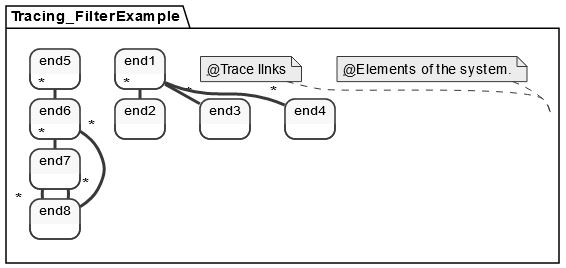
\includegraphics[width=.9\linewidth]{images/viz_filterexample.JPG}
	\caption{Example using the SysMLv2 filtering tool for trace annotations.}
	\label{fig:vizfilter}
\end{figure} 

\begin{figure}[ht]     
	\centering
	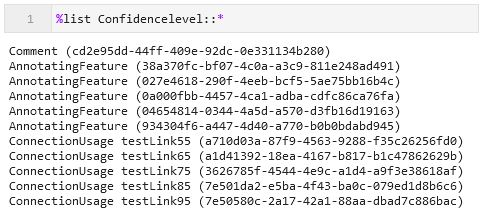
\includegraphics[width=.75\linewidth]{images/viz_filterexample_res.JPG}
	\caption{Filtering result: filtered annotations (\textit{i.e.,} satisfying a specific confidence).}
	\label{fig:vizfilterres}
\end{figure} 



The same process can (could) be used to "tag" links with specific types -- or any other pre-defined attribute. The implementation of the evaluation of expressions is unfortunately limited. As to this day, the use of strings of characters (\textit{String}) or of enumerations (\textit{enum}) in the definition of datatypes generates a compilation error. \Fig{fig:vizfiltererr} shows this limitation (the figure has been generated with JupyterLab, see \Sect{sec:artefacts}).

\begin{figure}[ht]     
	\centering
	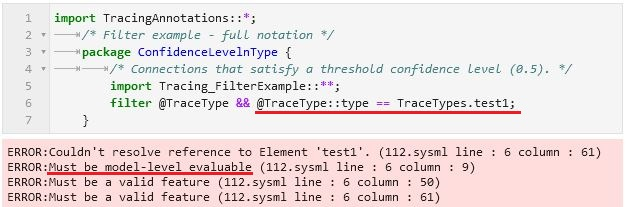
\includegraphics[width=.9\linewidth]{images/viz_filterexample_err.JPG}
	\caption{Filtering is not (yet) implemented for enumerations.}
	\label{fig:vizfiltererr}
\end{figure} 


\section{Conclusion}\label{sec:conclusion}
% \begin{descriptioncompact}
%     \item[Protocol] We propose a protocol to evaluate traceability solution
%     \item[Application] We show an application on Capra.
%     \item[Extension] We detail the extension of Capra as an example of Tracea integration.
%     \item[Limitations] We show Capra's design limitations
% \end{descriptioncompact}

This deliverable presents means to integrate quality traceability into SysMLv2 using Trace\textit{a}.
With Trace\textit{a} datatypes, SysMLv2 relationships can be annotated with valuable information related to their quality -- \textit{i.e.,} their \textit{trustability}. 
The degree of confidence as well as the information necessary to justify it can be associated to SysML links (connections) through metadata definition.


This integration is \textit{orthogonal}. It does not impact the structure of the language itself -- changes happen at the model level with new feature libraries, not at the metamodel level.
This allows the (re)use of the machinery supporting (meta)annotations and eases the (re)definition of tracing structures specific to a certain project or company. We showcase these benefits in one small example that also reveals the current limitations of SysMLv2's implementation.

The SST confirms that annotating features are valuable and salient artefacts in the development of SysML. They shall take more and more importance in the future releases. Work on the evaluation of expressions at the model level is highly required and will be part of the agenda of the fourth quarter of 2021. 
Finally, as a sign of encouragement, the SST invites us to further investigate in the direction we took. 

\section{Software artefacts}\label{sec:artefacts}
The software artifacts we have implemented have been uploaded to the Modelia Git repository and can be accessed at:
\url{https://github.com/modelia/tracea/3-sysml-integration}.

The file contains the two definitions presented above along with a simple example and a filtering usage example. Subfolders are \verb|/kerml| and \verb|/sysml| respectively to KerML and SysML versions.

SysML datatypes can be viewed in the JupyterLab of the SST. To do so, open the following link (\url{https://www.sysmlv2lab.com/}) in a web browser  and upload the code contained in \verb|/sysml/jupyterlab/TraceaTracingAnnotations.ipynb| from the Tracea Git repository. Its Markdown counterpart ($.md$) shows a \textit{Git readable} version of the Jupyter document.


%\appendix

%\cleardoublepage

%\section{Appendix}
%\includepdf[pages=-]{paper/MODELS_19_Submission.pdf}
%\label{sec:AppendixPaper}

%\input{sections/aa-appendix}

% Bibliography
%%%%%%%%%%%%%%%%%%%%%%%%%%%%%%%%%%%%%%%%%%%%%%%%%%%%%%%%%%%%%%%%%%%%%%

\cleardoublepage
\bibliographystyle{plain}
\bibliography{bib/strings-abbr,bib/trace-and-models,bib/uoc2020_tracea,bib/added}

% Clarifications
%%%%%%%%%%%%%%%%%%%%%%%%%%%%%%%%%%%%%%%%%%%%%%%%%%%%%%%%%%%%%%%%%%%%%%

% Print them only if the notes package is loaded (c@pagenode exists)
% and there are notes defined within the document (pnotesavechap > 0)

\makeatletter
\ifcsname c@pagenote\endcsname
\ifthenelse{\value{pnotesavechap}>0}{\cleardoublepage\printnotes}{}
\fi
\makeatother

%\makeback

\end{document}          
